%!Mode:: "TeX:System

%%%%%%%%%%%%%%%%%%%%%%%%%%%%%%%%%%%%%%%%%%%%%%%%%%%%%%%%%%%%%%%%%%%%%%%%%%%%%
%                                                                           %
%          LaTeX File for Doctor (Master) Thesis of ECNU                    %
%            华东师范大学博士(硕士)论文模板 ____lizb                      %
%                                                                           %
%%%%%%%%%%%%%%%%%%%%%%%%%%%%%%%%%%%%%%%%%%%%%%%%%%%%%%%%%%%%%%%%%%%%%%%%%%%%%




\documentclass[12pt,openany,a4paper,fancyhdr,twoside]{ctexbook}

%draft 选项可以使插入的图形只显示外框,以加快预览速度。
%\documentclass[11pt,a4paper,openany,draft]{book}
\usepackage{amsmath} 
\usepackage{amssymb}               % AMSLaTeX宏包 用来排出更加漂亮的公式
%\usepackage[CJKbookmarks]{hyperref}
\usepackage{url}
\usepackage[hidelinks]{hyperref}
\usepackage{shortvrb,indentfirst,ulem,makeidx}
\usepackage{fancyhdr}
\usepackage{graphicx}

\usepackage{rotating}


\usepackage{indentfirst,latexsym,colortbl,subfigure,clrscode}

%\usepackage[ruled,vlined,linesnumbered,]{algorithm2e}

\usepackage[linesnumbered,ruled,vlined,resetcount,algochapter]{algorithm2e}%[ruled,vlined]{  
\usepackage{algorithmicx}
\usepackage{listings}
\usepackage{algcompatible}
\usepackage{algpseudocode}


\renewcommand*{\algorithmcfname}{算法}

\newcommand{\clearPaperPage}{\clearpage}
%$\renewcommand{\clearPaperPage}{\cleardoublepage}




\SetKwInput{KwIn}{\textbf{输入}}
\SetKwInput{KwOut}{\textbf{输出}}
\SetKwInput{KwReturn}{\textbf{return}}


\usepackage{bibspacing}

\setlength{\bibitemsep}{2\baselineskip plus .05\baselineskip minus .05\baselineskip}


\usepackage{bm}                     % 处理数学公式中的黑斜体的宏包
\usepackage{amssymb}                % AMSLaTeX宏包 用来排出更加漂亮的公式
\usepackage{mathrsfs}
\usepackage[subnum]{cases}
\usepackage[numbers,sort&compress]{natbib}
\usepackage{hypernat}
\usepackage{geometry}
\usepackage{times}
\usepackage{fontspec}
%\usepackage{libertine}
\usepackage{libertineotf}
\usepackage{caption}
\usepackage{titletoc}
\usepackage{mathtools}

%\usepackage{chngcntr}
\counterwithout{footnote}{chapter}



%\usepackage{cite}
\usepackage{longtable,booktabs}
\usepackage{multirow}
\usepackage{subfigure}
\usepackage[subfigure]{tocloft}

\usepackage{float}
\usepackage{balance}
\usepackage {paralist}
\usepackage{bbding}
\usepackage{pgffor}

\usepackage{threeparttable}


%\usepackage{biblatex}
\makeindex
\pagestyle{fancy}

\renewcommand{\headrulewidth}{0.4pt}
\fancyfoot[CO,CE]{\thepage}

\renewcommand{\algorithmicrequire}{\textbf{Input:}}
\renewcommand{\algorithmicensure}{\textbf{Output:}}

\newtheorem{Def}{定义}

\newcommand{\yihao}{\fontsize{26pt}{36pt}\selectfont}           % 一号, 1.4 倍行距
\newcommand{\erhao}{\fontsize{22pt}{28pt}\selectfont}          % 二号, 1.25 倍行距
\newcommand{\xiaoer}{\fontsize{18pt}{18pt}\selectfont}          % 小二, 单倍行距
\newcommand{\sanhao}{\fontsize{16pt}{24pt}\selectfont}        % 三号, 1.5 倍行距
\newcommand{\xiaosan}{\fontsize{15pt}{22pt}\selectfont}        % 小三, 1.5 倍行距
\newcommand{\sihao}{\fontsize{14pt}{21pt}\selectfont}            % 四号, 1.5 倍行距
\newcommand{\banxiaosi}{\fontsize{13pt}{19.5pt}\selectfont}    % 半小四, 1.5 倍行距
\newcommand{\xiaosi}{\fontsize{12pt}{18pt}\selectfont}            % 小四, 1.5 倍行距
\newcommand{\dawuhao}{\fontsize{11pt}{11pt}\selectfont}       % 大五号, 单倍行距
\newcommand{\wuhao}{\fontsize{10.5pt}{15.75pt}\selectfont}    % 五号, 单倍行距


\renewcommand*{\bibfont}{\normalfont\normalsize\linespread{1}\selectfont}
\setlength{\bibitemsep}{\baselineskip}



%============================ 可以自定义文字块 ================================%


%交叉引用格式
\renewcommand\figureautorefname{图}
\renewcommand\tableautorefname{表}
\renewcommand\equationautorefname{公式}
\renewcommand{\algorithmautorefname}{算法}





\renewcommand{\contentsname}{\hfill\bfseries\Large 目录\hfill}   
\renewcommand{\cftaftertoctitle}{\hfill}

\renewcommand{\listtablename}{\hfill\bfseries\Large 表~~~~格\hfill} 
\renewcommand{\listfigurename}{\hfill\bfseries\Large 插~~~~图\hfill} 


\renewcommand{\listalgorithmcfname}{\centering\bfseries\Large 算~~~~法}
\newcommand*{\fullref}[1]{\textbf{\hyperref[{#1}]{第\ref*{#1}章~}}}


%=============================段前段后定义=============================% 


\def  \cftbeforetitleskip {45pt}
\def \cftaftertitleskip {25pt}
%% 目录部分
\setlength{\cftbeforetoctitleskip}{\cftbeforetitleskip}
\setlength{\cftaftertoctitleskip}{\cftaftertitleskip}

%% 图目录

\setlength{\cftbeforeloftitleskip}{\cftbeforetitleskip}
\setlength{\cftafterloftitleskip}{\cftaftertitleskip}

%% 表目录
\setlength{\cftbeforelottitleskip}{\cftbeforetitleskip}
\setlength{\cftafterlottitleskip}{\cftaftertitleskip}
%% 算法目录
%\setlength{\cftbeforeloatitleskip}{30pt}
%\setlength{\cftafterloatitleskip}{20pt}




\CTEXsetup[beforeskip=\cftbeforetitleskip]{chapter}
\CTEXsetup[afterskip=\cftaftertitleskip]{chapter}



%===============================概念定义===============================% 

\newcommand{\eat}[1]{}

\newcommand{\important}[1]{\CJKunderdot{\textbf{#1}}}

\newcommand{\TheisName}[0]{构建Android 动态函数调用图:RunDroid 的设计与实现}


\newcommand{\TheisNamePartOne}[0]{构建Android 动态函数调用图:}
\newcommand{\TheisNamePartTwo}[0]{RunDroid 的设计与实现}
\newcommand{\ecg}{拓展函数调用图}
\newcommand{\TheisNameEn}[0]{{\Large Building Android Dynamic Call Graph: }\\ Design and Implement of RunDroid}

\newcommand{\code}[1]{\textit{ #1 }}
\newcommand{\point}[1]{\subsubsection{\textbf{$\S$  #1 }}}
%\renewcommand{\point}[1]{\noindent{\textbf{$\S$  #1 }}}


\newcommand{\Line}[1]{ Line. #1}

\newcommand{\todo}[1]{\textcolor[rgb]{1,0,0}{\textbf{ #1 }}}
\newcommand{\question}[1]{\textcolor[rgb]{1,0,0}{\textbf{ #1 }?}}

\newcommand{\invoke}[2]{  $ (  #1 \to   #2)  $ }
\newcommand{\trigger}[2]{  $ (  #1 \hookrightarrow   #2)  $ }


\newcommand{\methodObjectRel}[3]{  $ (  #1 \stackrel{#2}{\longrightarrow}   #3)  $ }

\newcommand{\algrule}[1][.2pt]{\par\vskip.5\baselineskip\hrule height #1\par\vskip.5\baselineskip}



%%% ----------------------------------------------------------------------



%============================= 版芯控制 ================================%
\setlength{\oddsidemargin}{0.57cm}
\setlength{\evensidemargin}{\oddsidemargin}
\voffset-6mm \textwidth=150mm \textheight=230mm \headwidth=150mm
%\rightmargin=35mm
%                                                                       %


%============================= 页面设置 ================================%
%-------------------- 定义页眉和页脚 使用fancyhdr 宏包 -----------------%
% 定义页眉与正文间双隔线
\newcommand{\makeheadrule}{%
\makebox[0pt][l]{\rule[.7\baselineskip]{\headwidth}{0.4pt}}%
\rule[0.85\baselineskip]{\headwidth}{0.4pt} \vskip-.8\baselineskip}
\makeatletter
\renewcommand{\headrule}{%
{\if@fancyplain\let\headrulewidth\plainheadrulewidth\fi
\makeheadrule}} \makeatother

\newcommand{\adots}{\mathinner{\mkern 2mu%
\raisebox{0.1em}{.}\mkern 2mu\raisebox{0.4em}{.}%
\mkern2mu\raisebox{0.7em}{.}\mkern 1mu}}

\setmainfont{Times New Roman}
\dottedcontents{chapter}[1.5cm]{\xiaosi\heiti}{3.8em}{9.5pt}
\lhead{华东师范大学硕士专业学位论文}

\dottedcontents{section}[1.5cm]{\xiaosi\heiti}{2.8em}{9.5pt}
\lhead{华东师范大学硕士专业学位论文}

%=============================== 代码格式定义 ================================%


%% 辅助功能显示页边界
%\usepackage{showframe} % just for the example

\usepackage{etoolbox}




% thesis color scheme
\RequirePackage[table]{xcolor}
\definecolor{Strong Blue}{RGB}{6,64,194}
\definecolor{Dark Blue}{RGB}{6,46,139}
\definecolor{Night Blue}{RGB}{0,0,89}
\definecolor{Beige}{RGB}{219,212,192}
\definecolor{Dark Beige}{RGB}{185,170,129}
\definecolor{Night Beige}{RGB}{90,83,63}
\definecolor{Light Khaki}{RGB}{217,219,209}
\definecolor{Khaki}{RGB}{181,186,159}
\definecolor{Dark Khaki}{RGB}{113,117,99}
\definecolor{Light Red}{RGB}{214,124,118}
\definecolor{Red}{RGB}{212,24,14}
\definecolor{Night Red}{RGB}{105,18,12}
\definecolor{White}{RGB}{255,255,255}
\definecolor{Grey 1}{RGB}{238,238,238}
\definecolor{Grey 2}{RGB}{204,204,204}
\definecolor{Grey 3}{RGB}{170,170,170}
\definecolor{Grey 4}{RGB}{136,136,136}
\definecolor{Grey 5}{RGB}{102,102,102}
\definecolor{Grey 6}{RGB}{51,51,51}
\definecolor{Grey 7}{RGB}{33,33,33}
\definecolor{Black}{RGB}{0,0,0}
\definecolor{Frame Blue}{RGB}{0,85,128}
\definecolor{Frame Red}{RGB}{169,18,0}
\definecolor{Frame Green}{RGB}{55,143,23}
\definecolor{codegreen}{rgb}{0,0.6,0}
\definecolor{codegray}{rgb}{0.5,0.5,0.5}
\definecolor{codepurple}{rgb}{0.58,0,0.82}
\definecolor{backcolour}{rgb}{0.95,0.95,0.92}


\lstdefinestyle{mystyle}{
	frame=single,
	framexleftmargin=1.5em,
	commentstyle=\color{codegreen},
	keywordstyle=\color{magenta},
	numberstyle=\scriptsize ,
	stringstyle=\color{codepurple},
	basicstyle=\scriptsize,
	breakatwhitespace=false,         
	breaklines=true,                 
	captionpos=b,                    
	keepspaces=true,                 
	numbers=left,                    
	numbersep= 5pt,                  
	showspaces=false,                
	showstringspaces=false,
	showtabs=false,   
	xleftmargin=2em,       
	tabsize=2
}

% General style
\lstdefinestyle{normal}{
  aboveskip = 1.5em,
  backgroundcolor = \color{White},
   basicstyle = \ttfamily,
  belowskip = 1em,
   breakatwhitespace = false,
   breaklines = true,
   captionpos = b,
  commentstyle = \itshape\color{Dark Khaki},
  extendedchars = true,
  frame = lines,
  framerule = .6pt,
   framexleftmargin = 1em,
  framexrightmargin = 1em,
  gobble = 2,
  keywordstyle = \bfseries\color{Frame Blue},
  keywordstyle = [2]\bfseries\color{Frame Red},
  numbers = none,
  prebreak=\raisebox{0ex}[0ex][0ex]{\ensuremath{\hookleftarrow}},
  showspaces = false,
  showstringspaces = false,
  showtabs = false,
  stepnumber = 1,
  stringstyle = \color{Frame Green},
  tabsize = 2,
  upquote = true,
  xleftmargin = 1em,
  xrightmargin = 1em
}



% Cypher query language
\lstdefinelanguage{cypher} {
	keywords={start,create,set,delete,foreach,match,%
		where,with,return,skip,limit,order,by,asc,%
		ascending,desc,descending},
	morekeywords = {[2]type,id,length,nodes,rels,%
		relationships,abs,round,sqrt,sign,head,last,%
		tail,replace,left,right,substring,lower,upper,%
		ltrim,rtrim,trim,str,shortestpath,range,count,%
		sum,min,max,avg,collect,percentile\_cont,%
		percentile\_disc},
	sensitive = false,
	morecomment=[l]{//},
	morestring=[b]",
	morestring=[b]'
}


\lstset{style=mystyle}


%\CTEXsetup[beforeskip=0mm]{chapter*}
%\CTEXsetup[afterskip=3mm]{chapter*}



%=============================== 正文部分 ================================%

\begin{document}
\pagestyle{empty}
\setlength{\baselineskip}{25pt}  %%正文设为25磅行间距
\vspace{-2.0cm}
\noindent{{\zihao{4} {\large 2019} 届硕士专业学位论文}}\\
\vspace{-0.8cm}
\begin{flushleft}
\hspace{-0.5cm}
\renewcommand\arraystretch{1.5}
\begin{tabular}{l}
\noindent{{\zihao{4} 分类号:\underline{\qquad\qquad\qquad\qquad\qquad\qquad}}}  \\ 
\noindent{{\zihao{4} 密~~~~级:\underline{\qquad\qquad\qquad\qquad\qquad\qquad}}}\\ 
\end{tabular}
\hskip 0.9cm
\renewcommand\arraystretch{1.5}
\begin{tabular}{l}
\noindent{{\zihao{4} 学校代码:\underline{10269~~~\qquad}}}\\ 
\noindent{{\zihao{4} 学~~~~~~~号:\underline{51164500190}}}\\ 
\end{tabular}
\end{flushleft}


\vskip 1.8cm
\begin{center}
\scalebox{1.0}{
\includegraphics[width=2.7cm]{fig/ecnulogo.png}}  %原来为width=2.7cm
\hskip 0.5cm
\scalebox{1.0}{
\includegraphics[width=10.5cm]{fig/ecnulabel.png}}	%原来为width=10.5cm

%{\textbf{{\xiaoer East China Normal University}}}\\ \vskip 0.2cm
\vskip 0.5cm
%{\textbf{\erhao 硕~士~专~业~学~位~论~文}}\\ \vskip 0.2cm
%{\textbf{\xiaoer MASTER'S DISSERTATION(PROFESSIONAL)}}\\
\end{center}
\vskip 1.0cm

\begin{center}
%{\erhao \bf 论文题目:\underline{~基于ESHMARTE和ESHA的建筑物能源管理系统的建模与验证~}}\\
{\erhao \bf \underline{~\TheisNamePartOne}}\\
\vskip 0.3cm
{\erhao \bf \underline{~\TheisNamePartTwo~~}}
\end{center}

\vskip 1.0cm 
\begin{center}

\renewcommand\arraystretch{1.5}
\begin{tabular}{l}
{\sihao \bf 院\qquad\ \ \ 系:}\\ 
{\sihao \bf 专~业~名~称:}\\ 
{\sihao \bf 研~究~方~向:}\\ 
{\sihao \bf 指~导~教~师:}\\ 
{\sihao \bf 学位申请人:}
\end{tabular}
\begin{tabular}c
{\sihao \bf  计算机科学与软件工程学院}        \\ 
\hline {\sihao \bf 计\quad   算\quad   机\quad   技\quad   术}              \\ 
\hline {\sihao \bf 软件方法与程序语言}\\ 
\hline {\sihao \bf 徐\ 立\ 华\qquad    副\ 教\ 授}  \\
\hline {\sihao \bf 袁\quad \quad \quad   宇\quad  \quad \quad   杰}      \\ 
\hline
\end{tabular}


\end{center}

\vskip 2.0cm
\begin{center}
{\sihao 2018年11月}
\end{center}

\clearPaperPage



\pagestyle{empty}

\begin{flushleft}
	\footnotesize
	\begin{tabular}{l}
		\noindent{ Dissertation for master degree in 2019}  \\ 
		\noindent{  (Professional)}\\ 
	\end{tabular}
\hspace{104pt} 
	%\renewcommand\arraystretch{1.5}
	\begin{tabular}{lc}
	 University Code:  &  10269  \\ 
 Student ID: &    51164500190  \\ 
		%\noindent{{ 学\qquad 号:\underline{\anonymous{51164500190}{ *** }}}}\\ 
	\end{tabular}
\end{flushleft}

\vskip 2cm

\begin{center}
{\Huge $\mathbf{EAST}\,\mathbf{CHINA}\,\mathbf{NORMAL}\,
\mathbf{UNIVERSITY}$}
\end{center}

\vskip 3cm

\begin{center}
\bfseries{\scshape{\huge \TheisNameEn
}}\\
\end{center}

\vskip 3.5cm {\large
\begin{center}
\begin{tabular}{l}
Department:\\
Category:\\ 
Research Direction:\\
Supervisor:\\
Candidate:
\end{tabular}
\begin{tabular}c
\normalsize{{Department of Computer Science}}\\
\hline ~~~\anonymous{Master of Engineering}{***}  \\
\hline ~~~\anonymous{Software Method and Program Language}{***}\\
\hline ~~~ \anonymous{Associate Professor Lihua Xu}{***}\\
\hline ~~~  \anonymous{Yujie  Yuan}{***}\\

\hline
\end{tabular}
\end{center}}

\vskip 30mm

\begin{center}
{\Large Sept, 2018}
\end{center}


\clearPaperPage
\pagestyle{empty}
\centerline{\bf\Large 华东师范大学学位论文原创性声明}

\vskip 1cm

\normalsize \indent
郑重声明:本人呈交的学位论文《\TheisName》,是在华东师范大学攻读硕士/博士(请勾选)学位期间,在导师的指导下进行的研究工作及取得的研究成果。除文中已经注明引用的内容外,本论文不包含其他个人已经发表或撰写过的研究成果。对本文的研究做出重要贡献的个人和集体,均已在文中作了明确说明并表示谢意。

\vskip 1cm

\qquad\qquad{作者签名}:$\underline{\qquad\qquad\qquad }$
\qquad \qquad\qquad \mbox {日期}:\qquad 年 \qquad  月 \qquad  日


\vskip 1cm

\centerline{\bf\Large 华东师范大学学位论文著作权使用声明}

\vskip 0.8cm
《\TheisName》系本人在华东师范大学攻读学位期间在导师指导下完成的硕士/博士(请勾选)学位论文,著作权归本人所有。
本人同意华东师范大学根据相关规定保留和使用此学位论文,并向主管部门和学校指定的相关机构送交学位论文的印刷版和电子版;
允许学位论文进入华东师范大学图书馆及数据库被查阅、借阅;
同意学校将学位论文加入全国博士、硕士学位论文共建单位数据库进行检索,将学位论文的标题和摘要汇编出版,采用影印、缩印或者其它方式合理复制学位论文。


本学位论文属于(请勾选)

( ~)1.经华东师范大学相关部门审查核定的“内部”或“涉密”学位论文*,
于  ~~~~   年  ~~  月  ~~  日解密,解密后适用上述授权。

( ~ )2.不保密,适用上述授权。
$$\\ $$
\qquad\qquad \mbox{导师签名}:$\underline{\qquad\qquad\qquad\qquad}$
\qquad\qquad \mbox {本人签名}:$\underline{\qquad\qquad\qquad\qquad }$

\vskip 0.5cm

$\rightline{ \qquad 年 \qquad  月 \qquad  日 \qquad\qquad}$

\vskip 0.5cm

* “涉密”学位论文应是已经华东师范大学学位评定委员会办公室或保密委员会审定过的学位论文(需附获批的《华东师范大学研究生申请学位论文“涉密”审批表》方为有效),未经上述部门审定的学位论文均为公开学位论文。此声明栏不填写的,默认为公开学位论文,均适用上述授权)。


\clearPaperPage

\pagestyle{empty}
$$\\ \\ \\ $$

\centerline{\bf\Large $\underline{\mbox{\kaishu {{袁宇杰}}}\,\,}$硕士专业学位论文答辩委员会成员名单}

\vskip 10mm

\begin{center}\large
	\begin{tabular}{ |c|c|c|c| } 
		\hline
		\multirow{1}{25mm}{\tiny	} & \multirow{1}{30mm}{\tiny	} & \multirow{1}{48mm}{\tiny	} & \multirow{1}{25mm}{\tiny	} \\ 	
			\heiti  姓名 &\heiti  职称&\heiti  单位&\heiti  备注 \\ 
		\hline
		
		孙蕾	&副教授&	华东师范大学计算机系 &主席\\	\hline
		孙强	&副教授&	华东师范大学计算机系&\\		\hline
		周建武&	高级工程师&	中安电子信息科技有限公司&\\\hline
		
%		\anonymous{X~~x} & \anonymous{教授}  & \anonymous{华东师范大学} &  \textbf{主席} \\
	%	\hline
	%	\anonymous{X~~x} & \anonymous{教授}  & \anonymous{华东师范大学} &    \\
	%	\hline
	%	\anonymous{X~~x} & \anonymous{教授}  & \anonymous{华东师范大学} &   \\
	%	\hline
	\end{tabular}
\end{center}






\clearPaperPage
\pagenumbering{roman}
\pagestyle{plain}



\vspace{-2.5cm}
\chapter*{\zihao{2}\heiti{摘~~~~要}}
\vspace{-1cm}

\setlength{\baselineskip}{25pt}	

在Android,应用程序的逻辑分散在不同的代码段(例如方法、线程、组件等)中,这使得部分静态分析工具在分析时,得不到精确的结果。
为了帮助研究人员和开发人员了解Android 应用程序的执行过程,我们提供了RunDroid,一个用于还原Android应用程序运行时动态调用图的工具,进而帮助辅助静态工具提供更精确的程序分析结果。
RunDroid利用源程序代码插桩和运行时方法拦截的相结合的方式,捕获应用程序在应用层和系统层的方法执行信息,还原方法间的调用关系。
在此基础上,RunDroid利用对象和方法间的依赖关系,进一步还原方法之间的触发关系(例如),在调用图中展现运行过程中的Android特性。

另外,我们还将RunDroid和静态分析工具进行对比,分析两种技术在生成函数调用图上的优缺点。


\hspace{-0.5cm}
\sihao{\heiti{关键词:}} \xiaosi{Android,函数调用图,多线程,动态分析技术}


\clearPaperPage
\newpage
\vspace{-1cm}
\chapter*{\zihao{-2}\heiti{ABSTRACT}}
\vspace{-0.5cm}
%With the close coordination of calculation, communication and control technology, Cyber-Physical Energy System(CPES) realizes the organic integration of network infrastructure and physical infrastructure, which uses intelligent control technology to effectively manage system energy.
%CPES exists in complex physical environment and interacts with various random behaviors in the environment, in which continuous behaviors and discrete behaviors coexist. Therefore, it is stochastic and hybrid.
Cyber-Physical Energy System(CPES) is a kind of complex system with stochastic and hybrid features.
Smart building is a typical CPES, which changes the indoor environment parameters through the intelligent control of functional components, to provide a comfortable living environment for human beings. Also, it strives to reduce overall energy consumption of the system.

In the process of traditional development methods, systems are tested after designed and developed, and it is often too costly and time-consuming to modify systems. Thus, it is of great importance to use Model-Driven Development(MDD) method in order to find errors and inconsistencies in systems in the early stage. However, the modeling of complex CPESs such as smart buildings faces many challenges: 1) In view of the characteristics of CPES, combined with the features of smart buildings, how to effectively reuse the knowledge in this field, and guide the construction of design models? 2)How to modify the standard modeling language MARTE/UML to build system design models? 3)How to construct the executable models of CPES, and to analyze energy consumption and other properties?
To address the above problems, we propose a modeling and analysis method for energy consumption of smart buildings. The main contributions of this paper are as follows:

First of all, ontology of smart buildings is given based on the building information model and the main steps of ontology construction methods. The domain ontology includes the basic concepts of smart buildings, the relationships among concepts and the constraints. Besides, we also point out how to use it to guide system modeling.

Secondly, in view of CPES's energy-aware, stochastic and hybrid features, we extend the MARTE/UML modeling language: 1)Two typical stochastic behaviors are defined; 2)Data types and expressions in MARTE are extended; 3)The meta model of extended class diagrams, sequence diagrams, and state charts are presented to support modeling of energy consumption, stochastic, and hybrid behaviors.

Although MARTE/UML can realize the multi-view modeling of systems in an intuitive way, it is almost impossible to achieve model validation and evaluation because of its semi formal attributes. To solve this problem, we extend the Stochastic Hybrid Automata to Energy Stochastic Hybrid Automata(ESHA) based on energy consumption, and define its syntax and semantics. Besides, mapping rules from MARTE/UML state charts to ESHA are given, and the automatic model transformation is implemented. Based on our Modana tool and model verification tool UPPAAL-SMC, we present the implementation of the proposed method.

Finally, we study a specific case -- intelligent temperature control system with our proposed method. 
%With the help of domain ontology, the design model of intelligent temperature control system is built based on extended MARTE/UML language. Then the model is transformed to ESHA model automatically, and energy consumption is verified and evaluated with the UPPAAL-SMC tool.
The experimental results show that the method not only supports the complete modeling of smart buildings, but also can analyze system energy consumption and other properties with stochastic model checking technology.

{\sihao{\textbf{Keywords:}}} \textit{Smart Building, Domain Ontology, MARTE, 
Stochastic Hybrid Automata, Stochastic Model Checking.}



































\clearPaperPage

%\clearpage{\pagestyle{plain}\clearPaperPage}
%\textcolor[rgb]{1,1,1}{文本} 


%%%%%%%%%%%%%%%%%%%%%%%%%%%%%%%%%%%%%%%%%%
%                                                             目录                                                         %
%%%%%%%%%%%%%%%%%%%%%%%%%%%%%%%%%%%%%%%%%%

\setcounter{tocdepth}{2}
\tableofcontents

\clearpage
\let\origaddvspace\addvspace
\renewcommand{\addvspace}[1]{}

%%%%%%%%%%%%%%%%%%%%%%%%%%%%%%%%%%%%%%%%%%
%                                                             插图                                                         %
%%%%%%%%%%%%%%%%%%%%%%%%%%%%%%%%%%%%%%%%%%


%\setlength{\baselineskip}{30pt}  %%正文设为25磅行间距
\renewcommand{\cftfigpresnum}{图}
\setlength{\cftfignumwidth}{3em}

\listoffigures

%%%%%%%%%%%%%%%%%%%%%%%%%%%%%%%%%%%%%%%%%%
%                                                             表格                                                         %
%%%%%%%%%%%%%%%%%%%%%%%%%%%%%%%%%%%%%%%%%%
\clearpage
\renewcommand{\cfttabpresnum}{表}
\setlength{\cfttabnumwidth}{3em}

\listoftables


%%%%%%%%%%%%%%%%%%%%%%%%%%%%%%%%%%%%%%%%%%
%                                                             算法                                                         %
%%%%%%%%%%%%%%%%%%%%%%%%%%%%%%%%%%%%%%%%%%
\makeatletter
\renewcommand*{\l@algocf}[2]{\@dottedtocline{1}{1em}{2.3em}{算法 #1 }{#2}}
\makeatother

\listofalgorithms
\setlength{\baselineskip}{25pt}
 \renewcommand{\addvspace}[1]{\origaddvspace{#1}}




\clearPaperPage


%%%%%%%%%%%%%%%%%%%%%%%%%%%%%%%%%%%%%%%%%%
%                                                             插图                                                         %
%%%%%%%%%%%%%%%%%%%%%%%%%%%%%%%%%%%%%%%%%%



\let\origaddvspace\addvspace
\renewcommand{\addvspace}[1]{}
%\setlength{\baselineskip}{30pt}  %%正文设为25磅行间距
\renewcommand{\cftfigpresnum}{图}
\setlength{\cftfignumwidth}{3em}

\listoffigures
\clearPaperPage
%%%%%%%%%%%%%%%%%%%%%%%%%%%%%%%%%%%%%%%%%%
%                                                             表格                                                         %
%%%%%%%%%%%%%%%%%%%%%%%%%%%%%%%%%%%%%%%%%%

\renewcommand{\cfttabpresnum}{表}
\setlength{\cfttabnumwidth}{3em}

\listoftables

\clearPaperPage

%%%%%%%%%%%%%%%%%%%%%%%%%%%%%%%%%%%%%%%%%%
%                                                             算法                                                         %
%%%%%%%%%%%%%%%%%%%%%%%%%%%%%%%%%%%%%%%%%%


\makeatletter
\renewcommand*{\l@algocf}[2]{\@dottedtocline{1}{1em}{2.3em}{算法 #1 }{#2}}
\makeatother

\listofalgorithms
\setlength{\baselineskip}{25pt}
\renewcommand{\addvspace}[1]{\origaddvspace{#1}}





\clearPaperPage
\pagenumbering{arabic}
\pagestyle{fancy}
\fancyhead[LE,RO]{华东师范大学硕士专业学位论文}
\fancyhead[RE,LO]{ \leftmark}



\CTEXsetup[format+={\zihao{3}\heiti}]{chapter}
\CTEXsetup[format+={\raggedright\zihao{4}\heiti}]{section}
\CTEXsetup[format+={\zihao{-4}\heiti}]{subsection}


\setlength{\baselineskip}{25pt}  %%正文设为25磅行间距



% 在章首页添加页眉

\fancypagestyle{plain}{%
\fancyhead[LE,RO]{华东师范大学硕士专业学位论文}
\fancyhead[RE,LO]{ \leftmark}
}

\raggedbottom
%\banxiaosi
\xiaosi
\clearPaperPage


\chapter {绪论}
\label{chp:intro}

\section{研究背景}

在现在社会,人们和移动设备的关系越来越密切,衣食住行几乎都离不开手机。
每天,人们只需要打开手机上的应用,就可以完成几乎所有的生活需求,
从出行打车到在线订餐,从网上购物到房屋租赁。
移动应用已经深入到人们生活的方方面面。
以移动系统Android为例,根据著名网站statista的统计~\cite{GoogleP55:online}显示,Android官方应用平台 Google Play Store在2009年12月至2018年6月期间的应用数量变化如~\autoref{fig:app_number}所示。
Google Play Store于2008年8月上线,截止2018年3月,在Google Play Store 上架的应用已经超过330 万。
这个数字在2013年7月才刚刚突破100万。这也从一个侧面反映出最近几年移动应用迅猛的增长趋势。

\begin{figure*}[h]
	\centering
	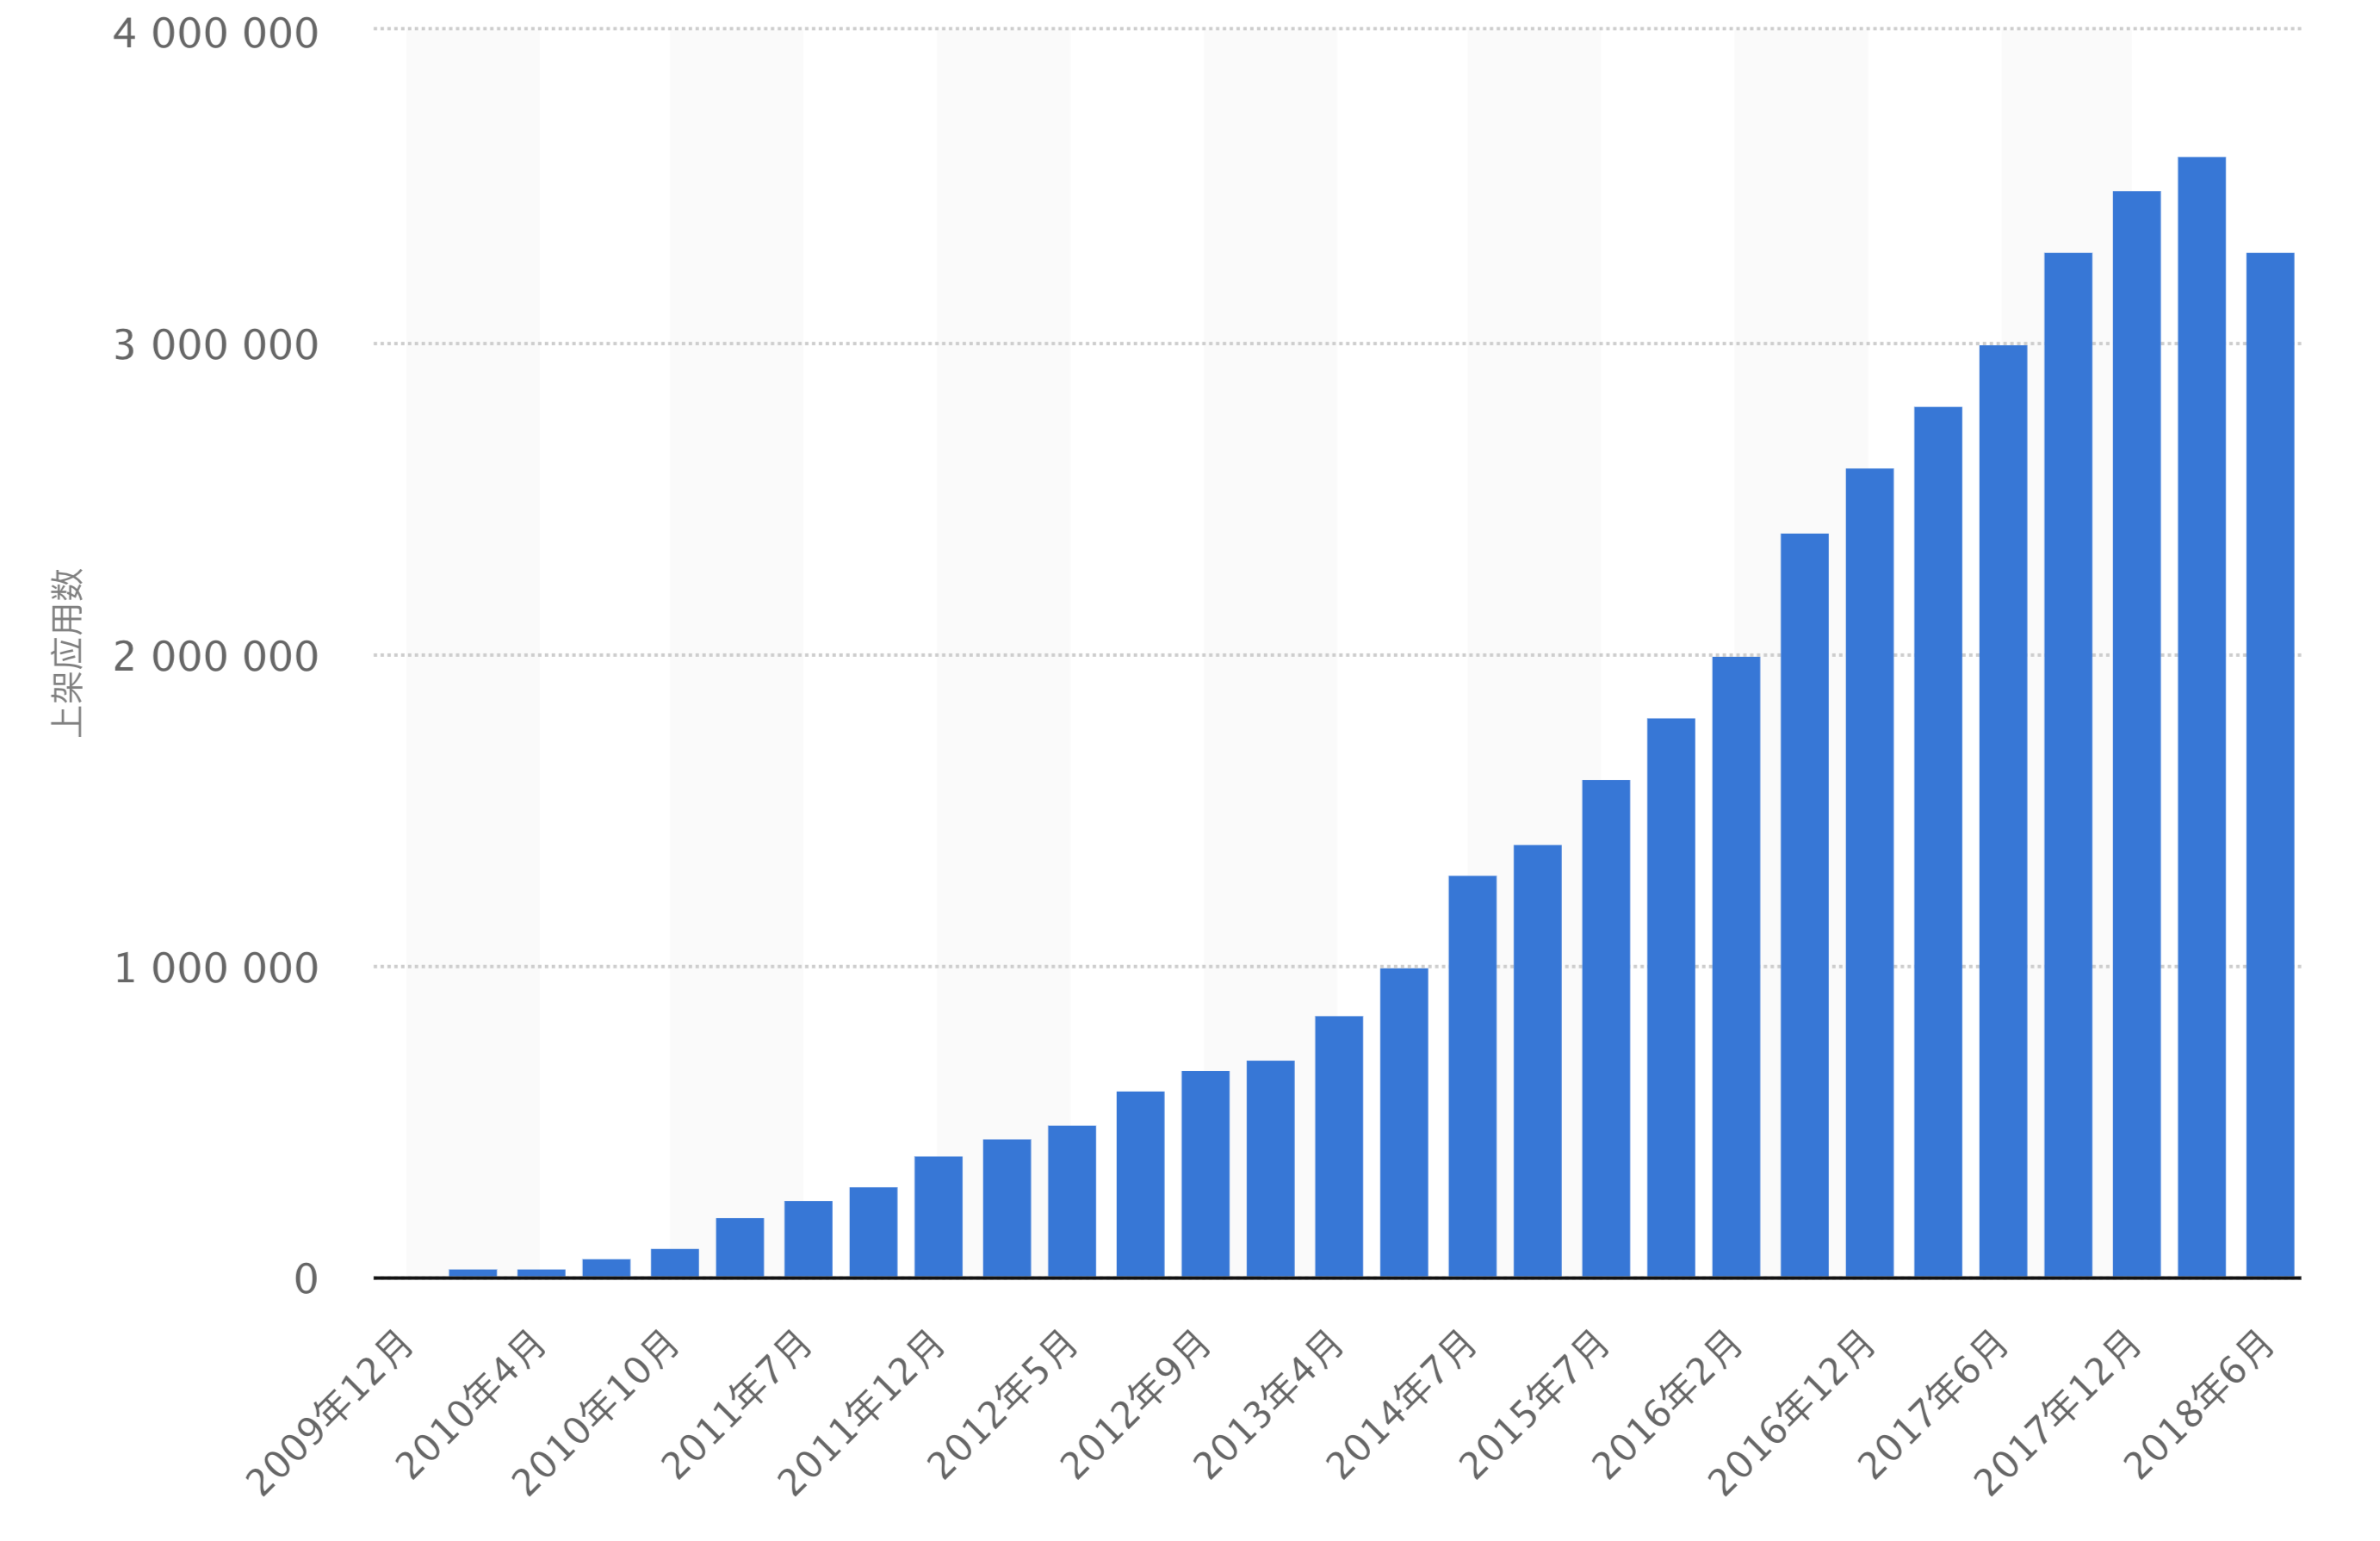
\includegraphics[width=\textwidth]{./Figures/app-numbers.png}
	\caption{Google Play Store上架的应用总数的变化趋势}
	\label{fig:app_number}
\end{figure*}


正因为移动应用迅猛的增长趋势,学术界和工业届的相关人员开始研究如何通过技术手段分析移动应用的代码内容,了解应用本身的运行时行为,进行相关学术研究和工业生产。
利用程序分析技术,研究人员对应用程序的项目相关源代码、配置文件或者二进制分发文件进行分析,监控程序的运行时行为,总结出应用程序相关特征。
结合具体应用场景,我们对这些特征进行归纳总结出相关规律,应用在应用分析、安全风险以及质量保障等领域,进一步提升应用程序的易用性、安全性和可靠性。

根据分析过程中是否需要运行目标程序,我们可以将这些技术手段分为静态分析技术和动态分析技术。
如果分析过程不依赖于目标程序的运行,这种分析技术称为静态分析技术,反之则为动态分析技术。
静态分析技术通常以二进制程序文件作为研究主体,结合相应的控制流分析、数据流分析技术、指针分析以及程序依赖分析,得出应用程序过程内的控制依赖和数据依赖(两者统称为程序依赖);
根据程序方法内相关函数/方法\footnote{在Java语言中,函数称为方法。在本文中,两者可以相互替换,不做区分。}调用,可以得到函数调用图、UML类图和序列图;
我们将程序依赖数据和函数调用图相结合,可以进一步得到过程间程序依赖~\cite{stafford2000formal},帮助研究人员了解程序整体层面的业务间的依赖关系,进行污点传播分析。
相反的,动态分析技术依赖目标程序的运行,通过修改目标程序的运行文件,搭建目标程序的运行环境,记录程序运行过程中相关操作信息,监控目标程序在运行过程中的状态变迁或指标变化,
进而得出程序在运行过程中的行为特定,帮助研究人员进行程序安全性分析,提升程序的质量可靠性。

但是,上述两种技术各有各的优劣。
静态分析技术有着较为扎实的理论基础,分析结果精确可靠,覆盖范围全面。
但是,静态分析技术在枚举所有情况时,往往会遇到状态爆炸的问题,具体实验效果受到实验运行环境的硬件条件和算法实现程度的限制。
而且,静态分析技术分析的问题依赖于外部环境(用户实时操作序列、手机所处环境因素,如温度等),分析得到的结果并不是非常准确。
动态分析技术却能解决这个问题,通过对程序运行状态的监控,研究人员可以了解程序的运行行为,掌握程序的安全性信息和可靠性信息。
但是,动态分析技术的缺点也非常明显:动态运行环境的搭建往往要设计到相关系统的源代码,构建系统的时间成本大,技术要求高。
另外,动态分析技术的分析结果往往只针对一次程序的运行过程,无法直接推广到其他运行情况。

Android应用程序的特性(例如,基于事件驱动的基础架构、面向组件的开发方式、高度依赖回调函数和多线程交互等)使得传统分析工具无法直接应用在Android程序上,对研究人员了解Android应用程序执行细节造成了一定的困扰。
为了解决这个问题,本文提出了一种静动态相结合的技术方案,通过程序源代码和运行环境进行预处理,获得程序的运行时信息,进而还原出Android应用程序的动态函数调用图。
在调用图中,除了方法调用关系,我们还提供了方法对象、方法间触发关系等信息,可以帮助研究人员补全函数关系,较为全面地了解应用程序运行时的状态变化。




\section{Android分析技术}

通常的,软件分析技术主要分为静态分析技术和动态分析技术两类。

\subsection{静态分析技术}
\todo{缩减此处,再添加3$\sim$5篇文献}
在不执行应用程序的情况下,静态分析技术通过对应用程序的源代码或者执行文件进行控制流分析和数据流分析,进而推断应用程序在运行过程中可能产生的行为。
这方面相关工具包括\cite{vallee1999soot,arzt2014flowdroid,AmanDroid,iccta,androguard:online}等。
Soot\cite{vallee1999soot}是传统的静态分析工具,其思路是将所有的Java字节码文件转化成一种中间语言Jimple,并在Jimple的基础上进行常规的控制流分析、数据流分析,理论上适用于所有可以在Java虚拟机上运行的语言(例如Scala、Groovy等等)的分析。
由于Android程序本身的字节码Davlik和Java字节码在格式上保持一致,因此,Soot也支持Android应用程序的静态分析。
但是,Soot在分析过程中没有考虑一些Android的特性难免会出现一些问题。
为此,德国达姆施塔特工业大学的Steven Arzt等人在Soot的基础上考虑Android程序中Activity的生命周期特性,推出了一个针对Android的静态分析工具FlowDroid\cite{arzt2014flowdroid},可以做到上下文、路径、对象、字段等层面上的敏感。
FlowDroid通过定义数据源点和数据泄漏点,在Android应用生命周期的基础上,可以实现数据流敏感的污点分析。
但其不足之处在于缺少跨组件通信的分析不考虑多线程调用问题。
在FlowDroid基础上,卢森堡大学的Li Li等人推出了IccTA\cite{iccta},利用跨组件通信分析工具IC3提取跨组件通信(Inter-Component Communication, ICC)的方法调用,并结合AndroidManifest.xml文件定义的Intent Filter信息,连接ICC两端的组件,克服了FlowDroid因缺少跨组件通信而导致的数据流上的缺失。
因为它是构建在FlowDroid之上的一个探测敏感信息泄露的,所以受限于FlowDroid的局限性。

Yang等人~\cite{yang2015static},利用静态分析技术,并将回调函数添加到控制流图(调用图)中,形成了回调控制流图(Callback control-flow gragh)。
实验结果显示,Yang的工作比Gator~\cite{rountev2014static}在控件监听器绑定上得到了更为准确结果。
%法国和意大利的学者~\cite{payet2012static}通过对Java字节码静态分析器Julia进行扩展,使得其支持对 Android 应用程序的静态分析;
%他们通过改写 Android 库中 Activity、LayoutInflater 等类的代码逻辑,规避了Android系统分析常见难点(如程序的事件机制,基于反射的视图加载等),
%实现了包括死代码检查、空指针检查在内的7种静态分析技术。



%由此可见,静态分析工具在分析过程中虽然可以对应用程序进行较为全面的分析,覆盖应用程序的所有代码,但由于缺少和程序执行过程相关的部分必要信息(应用程序的执行序列、和设备所处环境相关的传感器(如GPS、温度等)信息等),可能导致部分情况下分析结果的不精确。为了解决这一问题,研究人员提出了动态分析技术。


\subsection{动态分析技术}
\todo{缩减此处,再添加3$\sim$5篇文献}
% 为了解决这一问题,研究人员提出了动态分析技术。
和静态分析技术相对应,动态分析技术通过执行应用程序,获取程序运行过程的相关信息,从而实现对应的研究目的。
动态分析技术往往需要对运行环境做适当的修改或者调用特殊的系统接口,记录应用程序运行过程的关键信息,结合数据流追踪等技术,已记录应用程序的运行时行为。
这方面的工作代表包括\cite{chun2014taintdroid,droidbox:online,van2013dynamic,droidscope}等。
Enck等人提出的TaintDroid\cite{chun2014taintdroid},是一个高效的系统级的动态污点跟踪和分析系统。它通过修改Dalvik虚拟机,利用动态污点分析技术实时监控敏感数据的生成、传播和泄露,实现了变量层面、方法层面、文件层面的数据追踪。
此外,TaintDroid还支持跨进程通信(IPC)层面上的污点分析,因此可以精确分析出应用程序从消费者手机上获取和发布隐私信息的完整传播过程。
TaintDroid提供了较为完备的数据流分析技术,但是不支持控制流追踪,无法给出相关语句的执行路径。
DroidBox\cite{droidbox:online}在TaintDroid基础上,对Android Framework的部分API做了修改,可以记录一些开发人员感兴趣的API(例如文件读写、网络请求、SMS服务等)的调用,并提供分析结果的可视化。
同时,DroidBox还实现了应用程序的自动安装和执行,弥补了TaintDroid在软件测试自动化方面的不足。
和TaintDroid不同,TraceDroid\cite{van2013dynamic}采用的是另一种思路,利用字节码插装技术AspectJ,使得方法在执行时输出相应的日志信息。根据这些信息TraceDroid可以还原函数调用图,得到分析结果。
由于Aspect在进行字节码编织时引入的新的方法会导致方法数65K限制问题(即构建APK文件的过程中,方法总数超过65536,进而使得APK文件无法成功构建~\cite{Configur27}),因此该方案存在不稳定的情况。


另外,研究人员还用动态分析技术查找Android应用程序在运行时性能瓶颈。Android官方性能检测工具SimplePref~\cite{simpleperf:online}就是其中的一个代表。
SimplePref利用了Linux提供的系统接口\textit{pref\_event\_open},定时获取到性能监视单元的相关信息(例如cpu周期数、执行的指令数、缓存失效次数等)。
利用这些信息,SimplePref可以得到对应时刻的CPU状态,还原出各个方法的执行时间和对应的执行路径。
根据方法执行时间的长短和对应的执行路径,开发人员可以发现程序的性能瓶颈,进而通过对程序代码做出调整,提升程序的运行性能。
但是,该方法受到系统接口回调周期的影响,过于频繁的调度周期会使系统产生过大的开销,影响原有程序的执行;反之,则会丢失部分方法的执行信息。
而且,Android程序关心的性能瓶颈一般都位于主线程,而SimplePref会输出所有线程的执行信息,实际开销较大。
为此,Uber的Nanoscope~\cite{ubernanoscope:online}采用追踪(Trace)技术在定制化的系统Nanoscope OS中运行,在虚拟机解释执行目标方法前后输出相关Trace日志,进而得到性能报告。
相比SimplePref,Nanoscope只输出主线程相关的方法数据信息,大大减低了性能上的开销。
但是,nanoscope的局限性在于构建成本较高,需要配合特定的系统使用。




\subsection{分析技术的应用}

上述技术广泛运用在安全性分析、质量保障等领域。

\point{安全性分析:}

安全性分析包括隐私泄露、权限机制研究、恶意软件排查等。

%IOS Detecting privacy leaks in ios applications
\todo{缩减此处,再添加3$\sim$5篇文献}
为了弥补Android官方文档权限说明不完整的状况,多伦多大学的Kathy Au等人提出的PScout~\cite{au2012pscout}利用Soot对Android系统程序进行静态分析,
构建出Android系统的函数调用图,在调用图中标识权限相关的Binder跨进程调用,结合逆向可达性分析技术得出相关API接口以及对应调用路径上的所有权限检查的映射关系。
%相比其他类似工作,由于考虑了Android系统特性,PScout分析的到结果更加完整,但受到可达性分析的精度限制,存在部分错误的映射关系。
%此外,该团队对Android 2.1 $\sim$  4.0等四个版本的系统源代码进行了广泛的分析,就权限设计的冗余性、无文档说明API的权限要求、权限在Android系统升级的演变等多个研究问题进行深入的探讨。
在PScout的基础上,Rahul Pandita等人将目光聚焦到应用市场上,他们开发的\textsc{WhyPer}~\cite{pandita2013whyper}将自然语言处理技术(NLP)和传统静态分析技术相结合,
可以帮人们找出那些应用描述和实际使用到的权限不符的应用。
Wei Yang等人发现一部分恶意应用试图通过模仿正常应用的行为以防止被安全机构识别出来。%,例如恶意软件用到了和正常软件经常使用到的发送短信的功能,
不同的是恶意软件的行为一般在特定条件下(例如深夜)运行。
为此,Wei Yang等人提出了一种基于静态分析技术的解决方案AppContext~\cite{yang2015appcontext}:
在FlowDroid提供的函数调用图的基础上,AppContext结合Android常见的系统事件形成ICFG,提取出安全敏感行为的上下文,并利用SVM技术对这些信息进行机器学习,得到最终的安全检测模型。
实验结果显示,AppContext的准确率和召回率分别达到了87.7\%和95\%,这从一个侧面反映了安全敏感行为的恶意性与该行为的意图(通过上下文反映)更密切相关,验证之前提到的问题。
Zhemin Yang等人的AppIntent~\cite{yang2013appintent}利用静态分析技术提取应用程序的时间约束条件,再结合符号执行技术,最后得到一串可以导致用户信息泄露的序列。
Android应用程序中存在着大量的网络交互,因此,也有一部分研究Socket~\cite{Shao2016The,Jia2017Open,bu2017program}聚焦于移动应用的网络安全问题。



\point{质量保障}

伴随着Android应用程序的发展,研究人员也开始思考如何利用技术手段保障应用本身的质量。
%传统测试观点认为,在测试过程中,如果源代码的覆盖率可以维持在一个较高的水平,可在一定程度上可以覆盖
%其中,提高代码的覆盖率就是非常重要的一个方面。
这方面的工作包括提升软件在测试过程中的代码覆盖率\cite{azim2013targeted,yang2013grey,su2016fsmdroid,androidtest2}、程序错误的定位、分析与修复\cite{mirzaei2015exception,machado2013mzoltar,tan2018repairing,QingGaoASE15}以及变异测试\cite{MutationOperatorsAndroid,deng2015towards,linares2017enabling}等。
%t, most GUI testing techniques, e.g., random testing [39, 57], search-based testing [58, 60], and model-based testing [2, 3, 8, 78, 85]
工作\cite{azim2013targeted}利用静态分析工具SCanDroid得到静态Activity迁移图,并结合基于目标探索策略和深度优先探索策略进而达到了较好的Activity覆盖率。
Wei Yang等人的工作\cite{yang2013grey}通过对APP的状态进行建模,在深度优先算法的基础上,使得程序在当前状态无可再遍历状态的情况下进行回溯。
相比传统的深度优先算法,Wei Yang的工作对应的时间开销更小,效率更高。
此外,Stoat\cite{su2016fsmdroid,androidtest2}利用静态、动态分析技术标识出程序本身的状态和事件,从应用中抽象出有限状态机(FSM)模型。
基于该模型,Stoat进行模型变异、测试用例生成与执行、模型迭代,使得应用程序的覆盖率相比之前工作\cite{hao2014puma,amalfitano2015mobiguitar}提升了17$\sim$31\%。
工作\cite{mirzaei2015exception,machado2013mzoltar}等将传统软件的错误定位技术——基于频谱的错误定位技术(spectrum-based fault location,SBFL)运用在Android应用上,取得了不错的成绩。
工作\cite{tan2018repairing,QingGaoASE15}等主要聚焦如何在Android应用程序出现问题时,根据异常的堆栈信息结合软件变异技术或者问答网站生成补丁代码,实现程序的自动修复。
Lingling Fan等人的工作~\cite{fan2018large}通过开源社区中应用的issue解析分析,从异常种类(应用异常、系统异常、库(Library)异常)、系统异常分类、错误检查工具以及错误修复方式等若干方面进行较为深入的分析、探讨和总结。

\eat{

\point{应用分类:}

Simapp~\cite{chen2015simapp}

mobile app tagging ~\cite{chen2016mobile}

}


% 例如错误定位、自动化分析、profiling等

\section{本文的主要工作}

本文的主要研究工作包括以下:

1)	调研最近几年Android应用分析领域的静动态分析工具,了解各项工具的优劣以及相关的应用案例。

2)	提出并实现Android动态函数调用图构建系统RunDroid,包含传统函数调用图的构建以及在此基础之上的多线程函数调用关系的构建。

3)	将RunDroid和静态分析工具进行对比,分析两种技术在生成函数调用图上的优缺点。


%\todo{对上述系统设计对应的实验方案,评估对应的实验效果。}

\section{本文组织结构}

本文共分为六章,环绕着Android动态函数调用图构建系统的设计与实现展开,各章节内容如下:

第一章:主要介绍了本文的主要研究背景、相关工作以及主要工作内容。

第二章:从Android的体系结构出发,介绍了和Android系统相关的背景知识。

第三章:方法和对象的关系、方法间关系、调用图等几个方面介绍本文用到的概念做了符号化的定义,并结合文章的例子对这些概念做了进一步的说明。

第四章:从系统功能、相关挑战、技术路线、技术选型、模块实现等若干方面介绍RunDroid的设计与实现。

第五章:将展示RunDroid系统生成的函数调用图的运行结果,并对函数调用图进行详细的阐述。

第六章:对本文工作进行总结,并对下一步工作进行展望。



\clearPaperPage


\chapter{Android系统相关背景介绍 }  
\label{chp:background}


本章首先会简要介绍Android系统架构,其次会对Android中的Activity组件做基本介绍,接着会着重介绍Android中常见的两种多线程交互方式,最后将指出本文系统在实现上的难点。

\section{Android系统结构介绍}

Android是基于Linux内核开发的的开源操作系统,隶属于Google公司,主要用于触屏移动设备如智能手机、平板电脑与其他便携式设备,是目前世界上最流行的移动终端操作系统之一。
在系统架构上,Android自下到上,可以分为四层:Kernel层、Library和Android Runtime(Dalvik/ART)、Framework、Application等,如~\autoref{fig:Android-Framework}所示。
Kernel层是硬件和软件层之间的抽象层,主要是设备的驱动程序,例如:显示驱动、音频驱动、蓝牙驱动、Binder IPC驱动等。
Library和Android Runtime(Dalvik/ART): Library,顾名思义就是向上层提供各种这样的基础功能,例如SQLite数据库引擎,Surface Manager显示系统管理库。
Android Runtime主要是运行Android程序的虚拟机,在不同版本的系统上对应着不同的虚拟机,例如在Android 5.0及以上是ART,而在Android 4.3及以下是Dalvik,而Android 4.4两者都有。
Framework层主要是系统管理类库,包括Activity的管理,消息通知的管理;同时,它是Application的基础架构,为应用程序层的开发者提供了API,其存在简化了程序的开发。
而Application就是我们平时接触的应用,开发人员公国调用底层Framework提供的API实现相应的接口。

虽然Android应用程序是使用Java语言开发的,但是它和传统的Java程序有着很大的不同,具体有如下几点:

\begin{figure*}[!h]
	\centering
	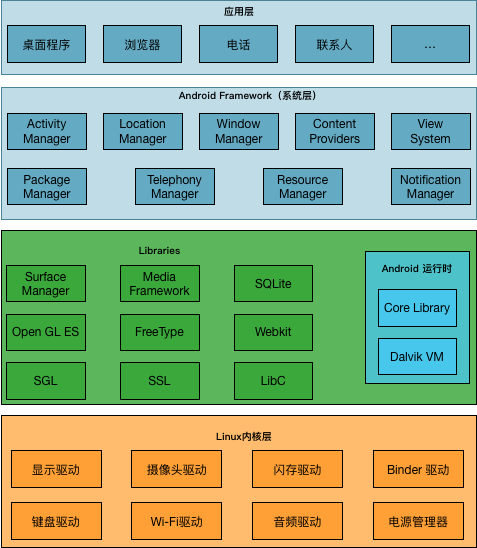
\includegraphics[width=0.8\textwidth]{./Figures/Android-Framework.png}
	\caption{Android系统框架图}
	\label{fig:Android-Framework}
\end{figure*}


\textbf{基于事件驱动的编程模型:}
在设计上,Android应用程序的开发架构采用的是事件驱动架构。在开发过程中,没有传统程序中入口函数Entry Point的概念。
应用程序中通用的业务逻辑(例如应用程序如何启动退出、应用的窗口如何创建销毁等)存在于Android Framework中。
%这也使得Android应用程序的分发文件(即APK文件)相对较小。

\textbf{面向组件的开发方式:}
Android程序中较为常见的是组件(Component,例如Activity、Service、Content Provider、Broadcast Receiver),它是应用程序运行的最小单元,受到Android Framework的直接调度。
开发人员通过继承这些组件,重写对应的生命周期函数,已实现对应的业务需求(界面的布局、页面状态的保存等),而这些组件的生命周期由Framework调度完成。

\textbf{大量逻辑实现依赖于回调函数和多线程通信:}
由于Android应用程序采用的是基于单线程消息队列的事件驱动架构,因此,界面相关的操作只允许出现在主线程(UI Thread)中,耗时操作只能在工作线程(Worker Thread)中进行。
通常的,开发人员往往会借助回调函数处理控件的响应事件,利用多线程交互串联界面相关操作和耗时操作,完成对应的业务。


\section{Android中的Activity}



在Android应用程序运行过程中,Activity向用户展示图形界面,响应用户的反馈,和其他组件一同完成相关业务,扮演着最为重要的作用。%\cite{Activity2:online}。
由于Android应用程序在架构选型上采用了事件驱动模型,为了便于协调应用内部状态的管理,Android组件通常有生命周期的概念,Activity也不例外。

Android系统根据Activity 在运行时和用户的反馈将其状态分为以下四种:



\begin{itemize}
		\setlength{\itemsep}{-5pt}
		
	\item 运行态:在该状态下, Activity处于页面最前端时,用户可以与Activity进行交互。
	一般的,我们看到Activity均处于这个状态。
	
	\item 暂停态:在该状态,Activity仍然可见,但是失去了窗口的焦点。
	当一个Activity之上出现非全屏的窗体(例如对话框)时,Activity就处于这个状态。
	处于暂停状态的Activity仍处于存活状态,保存着所有的内存数据。%,只有当系统内存极度紧张时,才有可能被系统杀死回收。
	
	\item 停止态:当一个Activity被其他的Activity遮挡时,处于这个状态。
	处于该状态的Activity仍然可以保留所有的状态,只是对用户不可见。
	系统在需要内存的情况下,可以采用相应的策略对Activity进行杀死回收操作。
	
	\item 终止态:当Activity处于暂停态或者停止态时,系统由于内存原因可能会将上述两种Activity杀死回收。
	处于该状态下的Activity将不能直接恢复。
\end{itemize}



\begin{figure*}[!ht]
	\centering
%	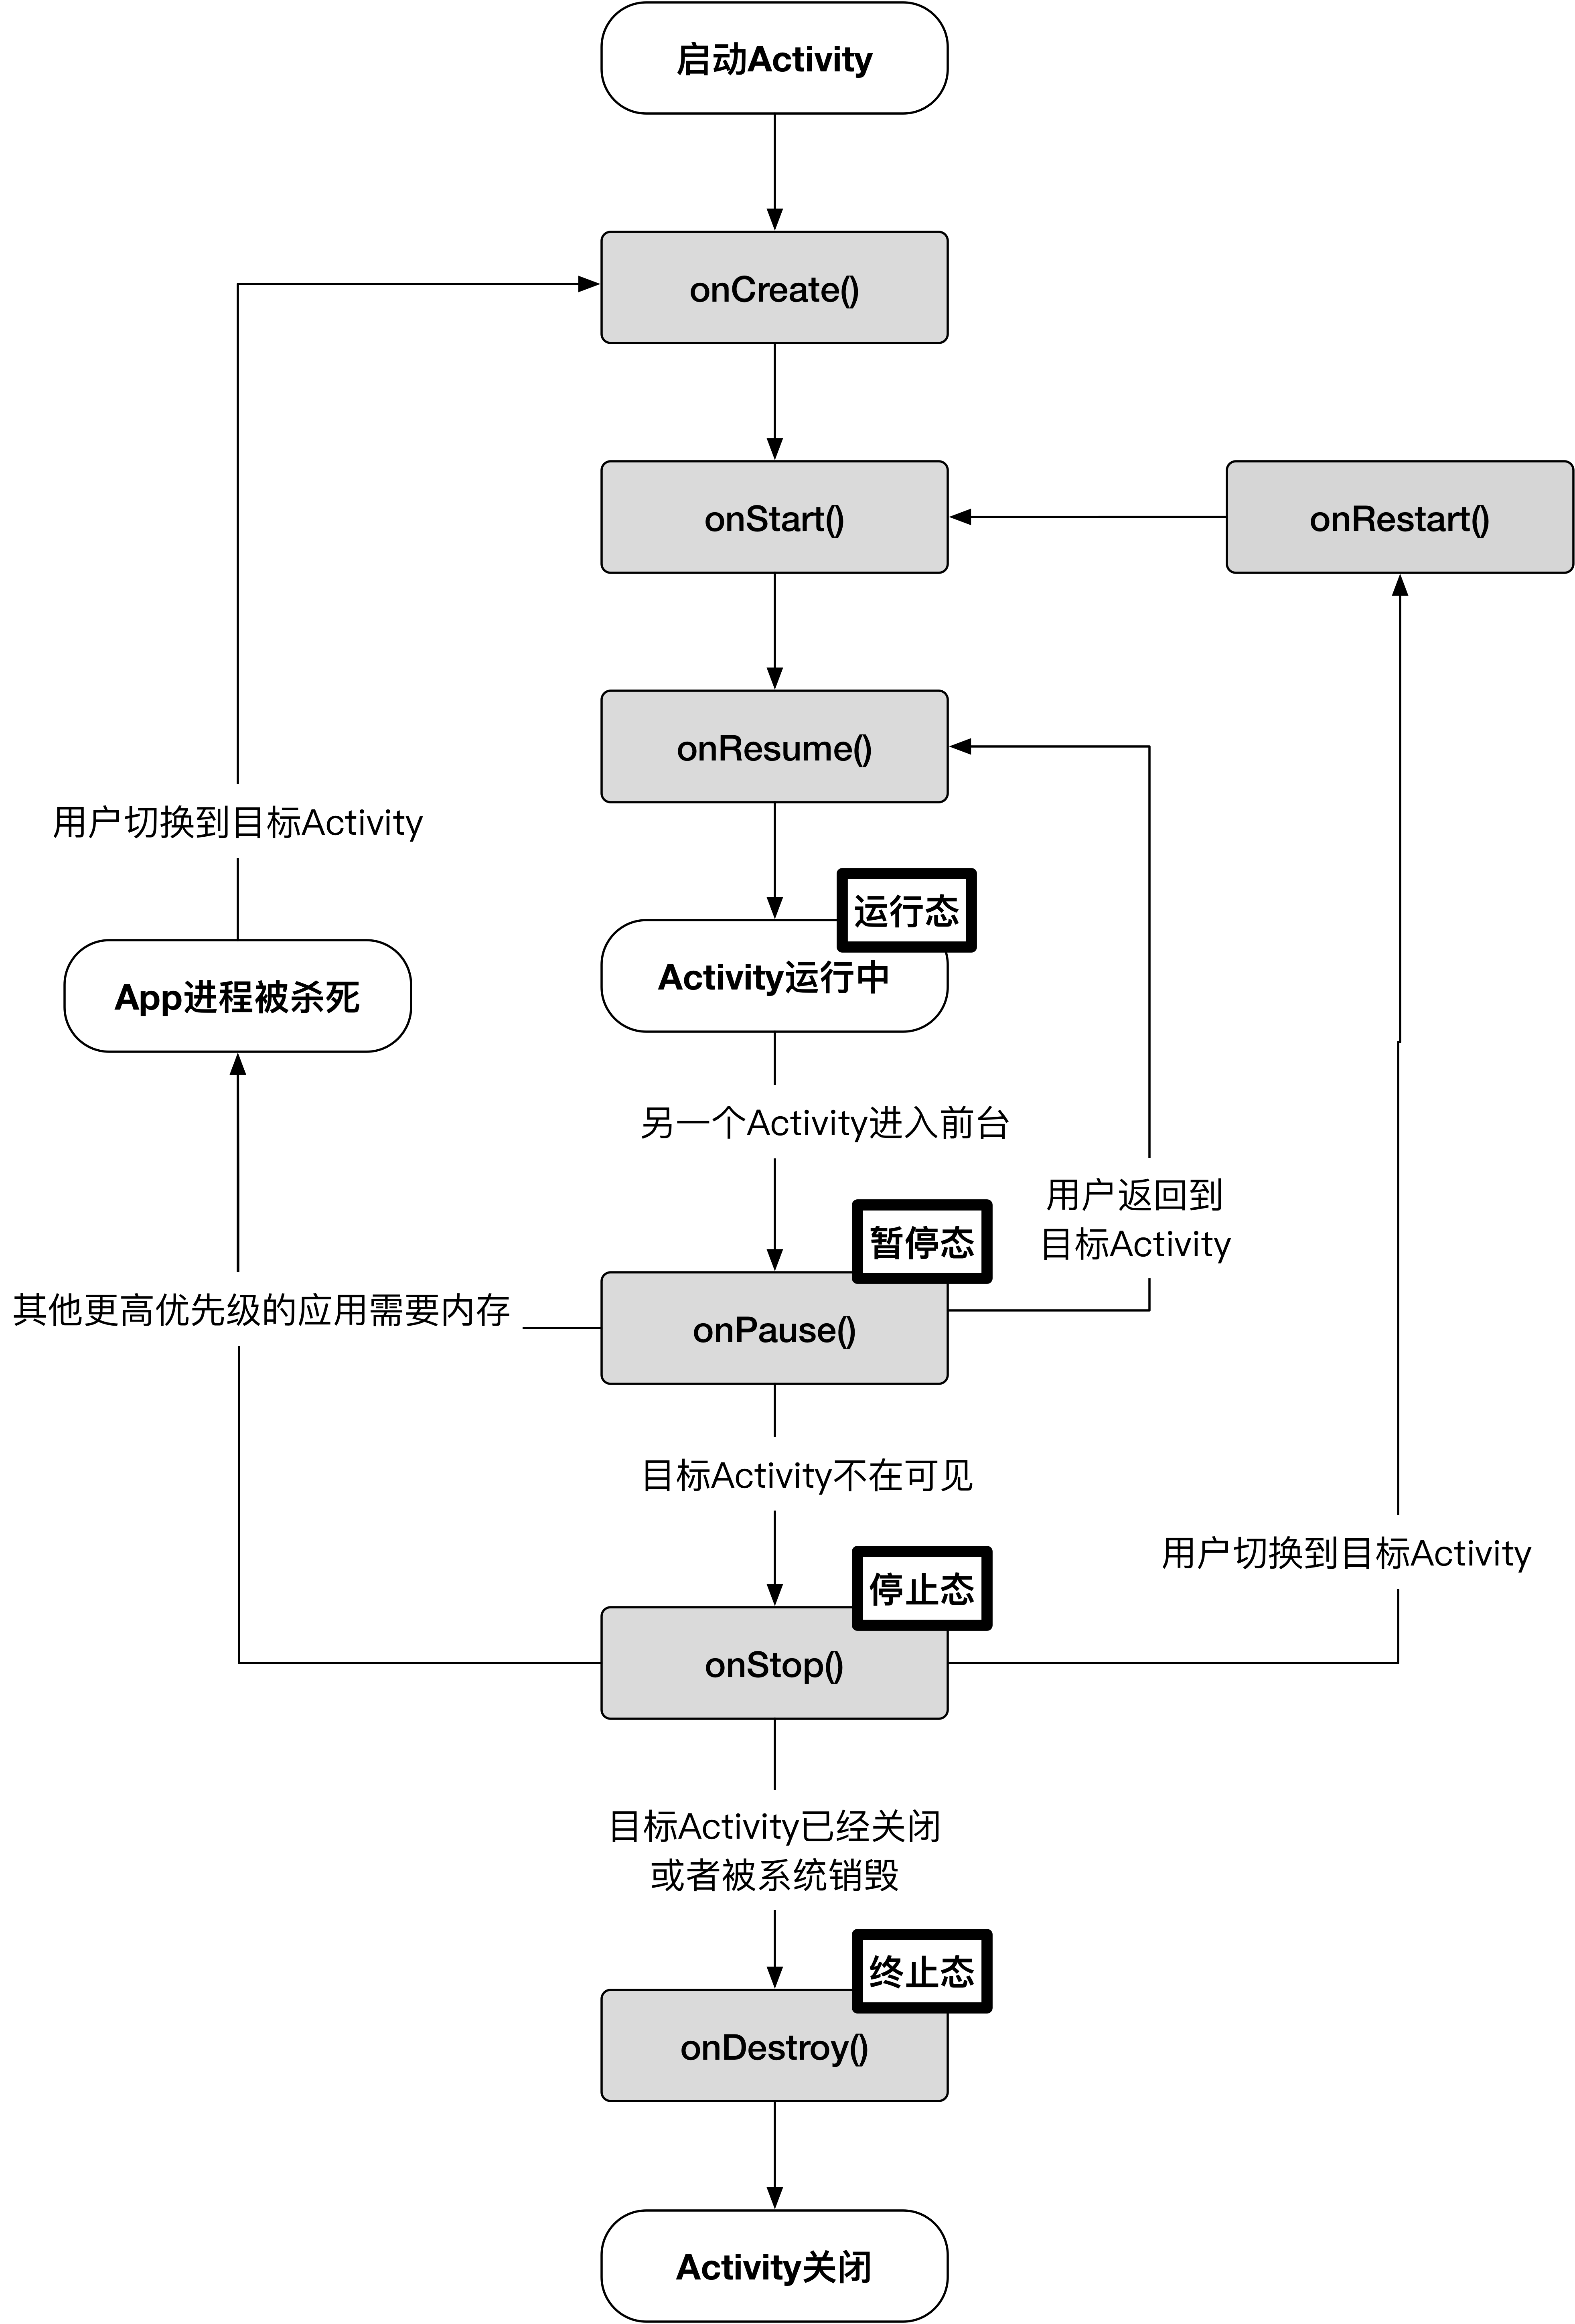
\includegraphics[width=0.9\textwidth]{./Figures/Activity-lifecycle.png}
	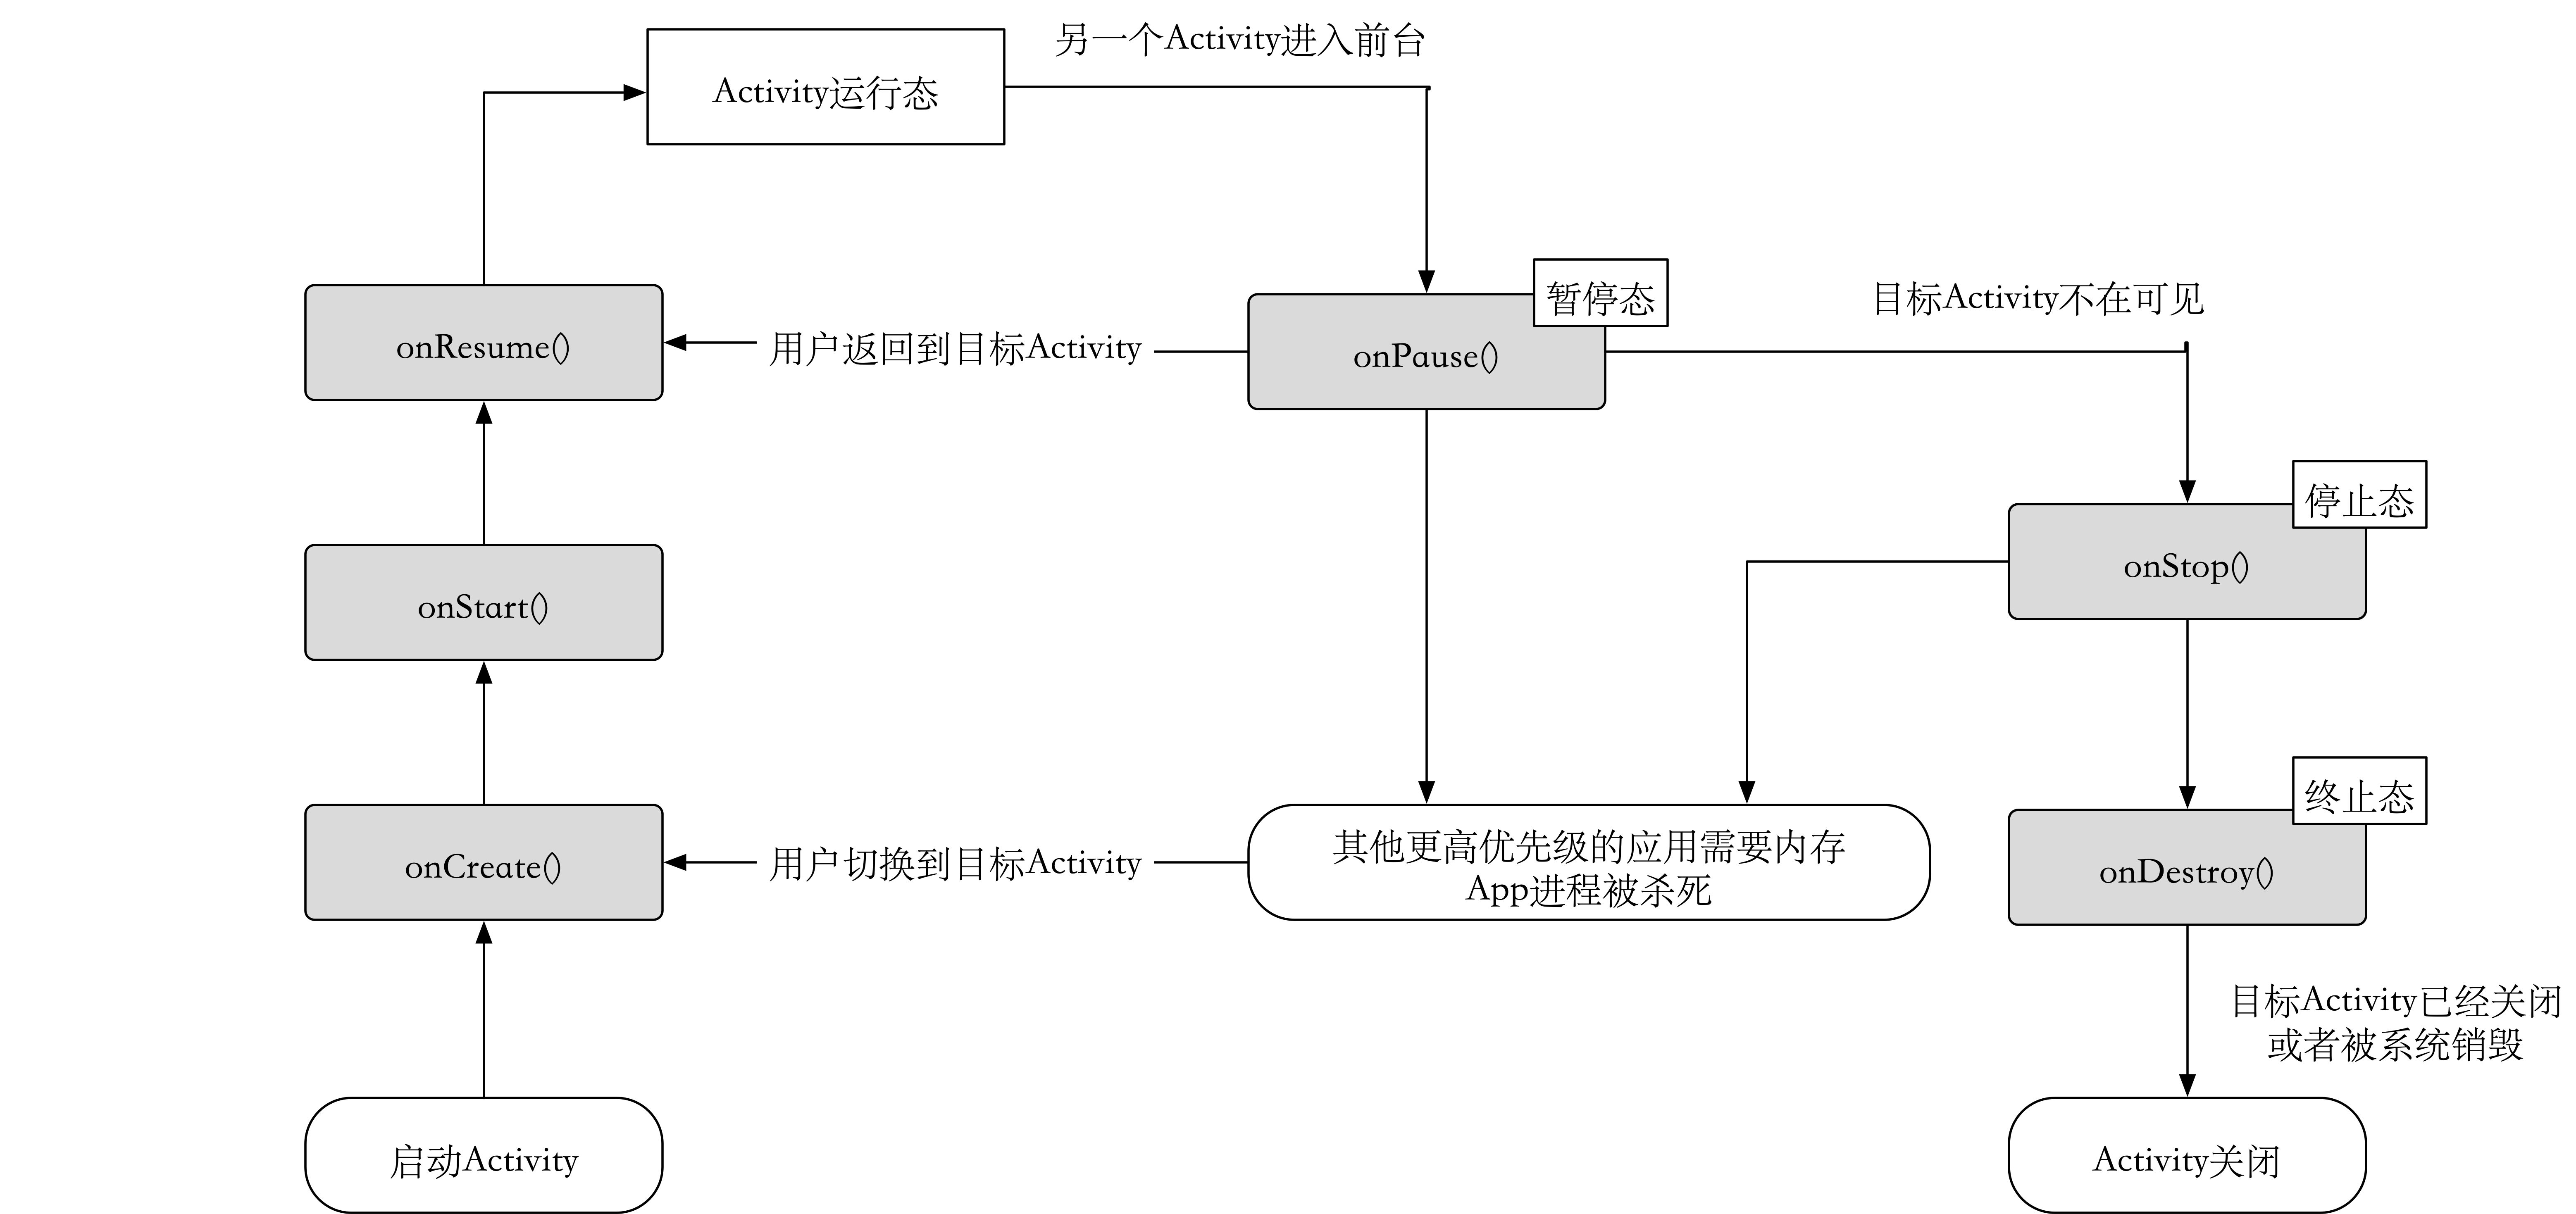
\includegraphics[width=0.9\textwidth]{./Figures/Activity-lifecycle-Landscape.png}
	
	\caption{Activity的生命周期}
	\label{fig:Activity-lifecycle}
\end{figure*}

Activity的生命周期就是以上状态之间的跳转,受到Activity在运行时的内存分布、环境状态以及业务逻辑的影响,由Android系统直接负责调度。
和\code{Activity}生命周期相关的方法包括\code{onCreate()}、 \code{onStart()}、\code{ onResume()}、 \code{onPaused()}、 \code{ onStop()}和\code{onDestroy()}等,方便开发人员在\code{Activity}的状态发生变化时对程序的运行时数据和应用状态做适当的处理操作。
\code{Activity}的生命周期如\autoref{fig:Activity-lifecycle}所示:



当用户点击应用图标,系统启动应用程序后,系统会创建、启动Activity并使之可以和用户进行交互。
在这个过程中,\code{onCreate()}、\code{onStart()}、\code{onResume()}等方法被回调,Activity最终处于运行态;


当Activity被其他窗体遮挡,只失去焦点,仍处于可见状态时,Activity的状态从运行态变成暂停态,\code{onPause()}方法会被回调;当Activity重新获得焦点时,\code{onResume()}方法会被调用;

当Activity切换到另一个Activity时,原来Activity将从运行态变为停止态,\code{onPause()}、\code{onStop()}等方法会被调用;
当返回原来的Activity时,\code{onStart()}、\code{onResume()}等方法会被调用,Activity从暂停态变为运行态。
%将从从运行态变成暂停态时,Activity只失去焦点,仍处于可见状态,\code{onPause()}方法会被回调;当Activity重新获得焦点时,\code{onResume()}方法会被调用;

当用户点击“返回键”返回到桌面时,Activity会失去焦点,在用户的视野中消失,直至被系统回收,
对应的状态也从运行态经暂停态、停止态,变为终止态,期间\code{onPause()}、\code{onStop()}、\code{onDestroy()}等方法被回调。

\eat{
当用户从一个界面回到原来的界面时,原来的Activity从停止态重启,出现在设备界面上,获得交互焦点,
\code{onStart()}、\code{onResume()}等方法被回调;
}


\section{Android中的多线程交互}
Android系统在架构设计上采用了事件驱动架构。在多线程并发访问时,若UI控件对于各线程均是可见的,并发对控件做读写操作会使控件处于不可预期的状态;
若贸然对控件使用锁机制,访问控件的各个线程之间存在竞争关系,阻塞相关线程业务逻辑的执行,使得应用变得复杂低效。
%上述情况对于应用程序都是不可接受的。
为了避免此类低效率问题,Android系统在设计事件驱动架构时,采用了单线程的消息队列,即只允许在UI线程(也称为主线程,Main Thread)进行界面更新操作,不允许在其他线程(也称为工作线程,Worker Thread)进行界面更新操作。
另外,为了保证应用程序界面渲染和事件响应的及时性,任何在主线程上产生的耗时操作(例如加载磁盘上的图片、网络请求等)都是不被允许的。
换而言之,当应用程序需要进行耗时操作时,这个操作往往会在一个新的线程中执行,而不是在主线程中。


Android系统架构中的单线程消息队列以及主线程的非阻塞性,使得界面更新和耗时操作分散在不同的线程中。
只因如此,多线程交互在Android应用程序开发过程中十分常见。
从整体上,系统提供的交互方式分为两种:基于Java的多线程交互和基于Handler的交互方式。%\cite{androidSourceCode}。

\subsection{基于Java的多线程交互}

由于Android系统提供的API接口兼容Java多线程相关的部分API,因此,在Android系统中,开发人员可以采用和Java应用相同的调用方式启动工作线程,并在对应的线程上完成业务逻辑。
但是,Java API只能实现业务逻辑从原有线程转移到新的工作线程上,不能重新返回到主线程上。
为此,Android系统在Java API的基础上还提供了API \code{void runOnUiThread (Runnable runnable) }。
该API可以帮助开发人员将业务逻辑的执行从工作线程转移到主线程上,该API也符合Android只允许在主线程上更新界面这一基本设计原则。
但是,该API也存在着一些弊端,例如\code{runOnUiThread(Runnable)} API的定义位于类\code{android.app.Activity},这也就意味着在Android组件Service中进行耗时操作时,无法通过该API返回到主线程;同时基于接口的函数参数定义方式对于跨线程的参数传递也不是十分友好。
为此,Android提供了基于Handler的多线程交互方式。

\subsection{基于Handler的多线程消息调度}

为了满足开发人员多样化的业务在多线程间的切换,Android提供了基于Handler消息调度的多线程交互方式。



\begin{figure*}[h]
	\centering
	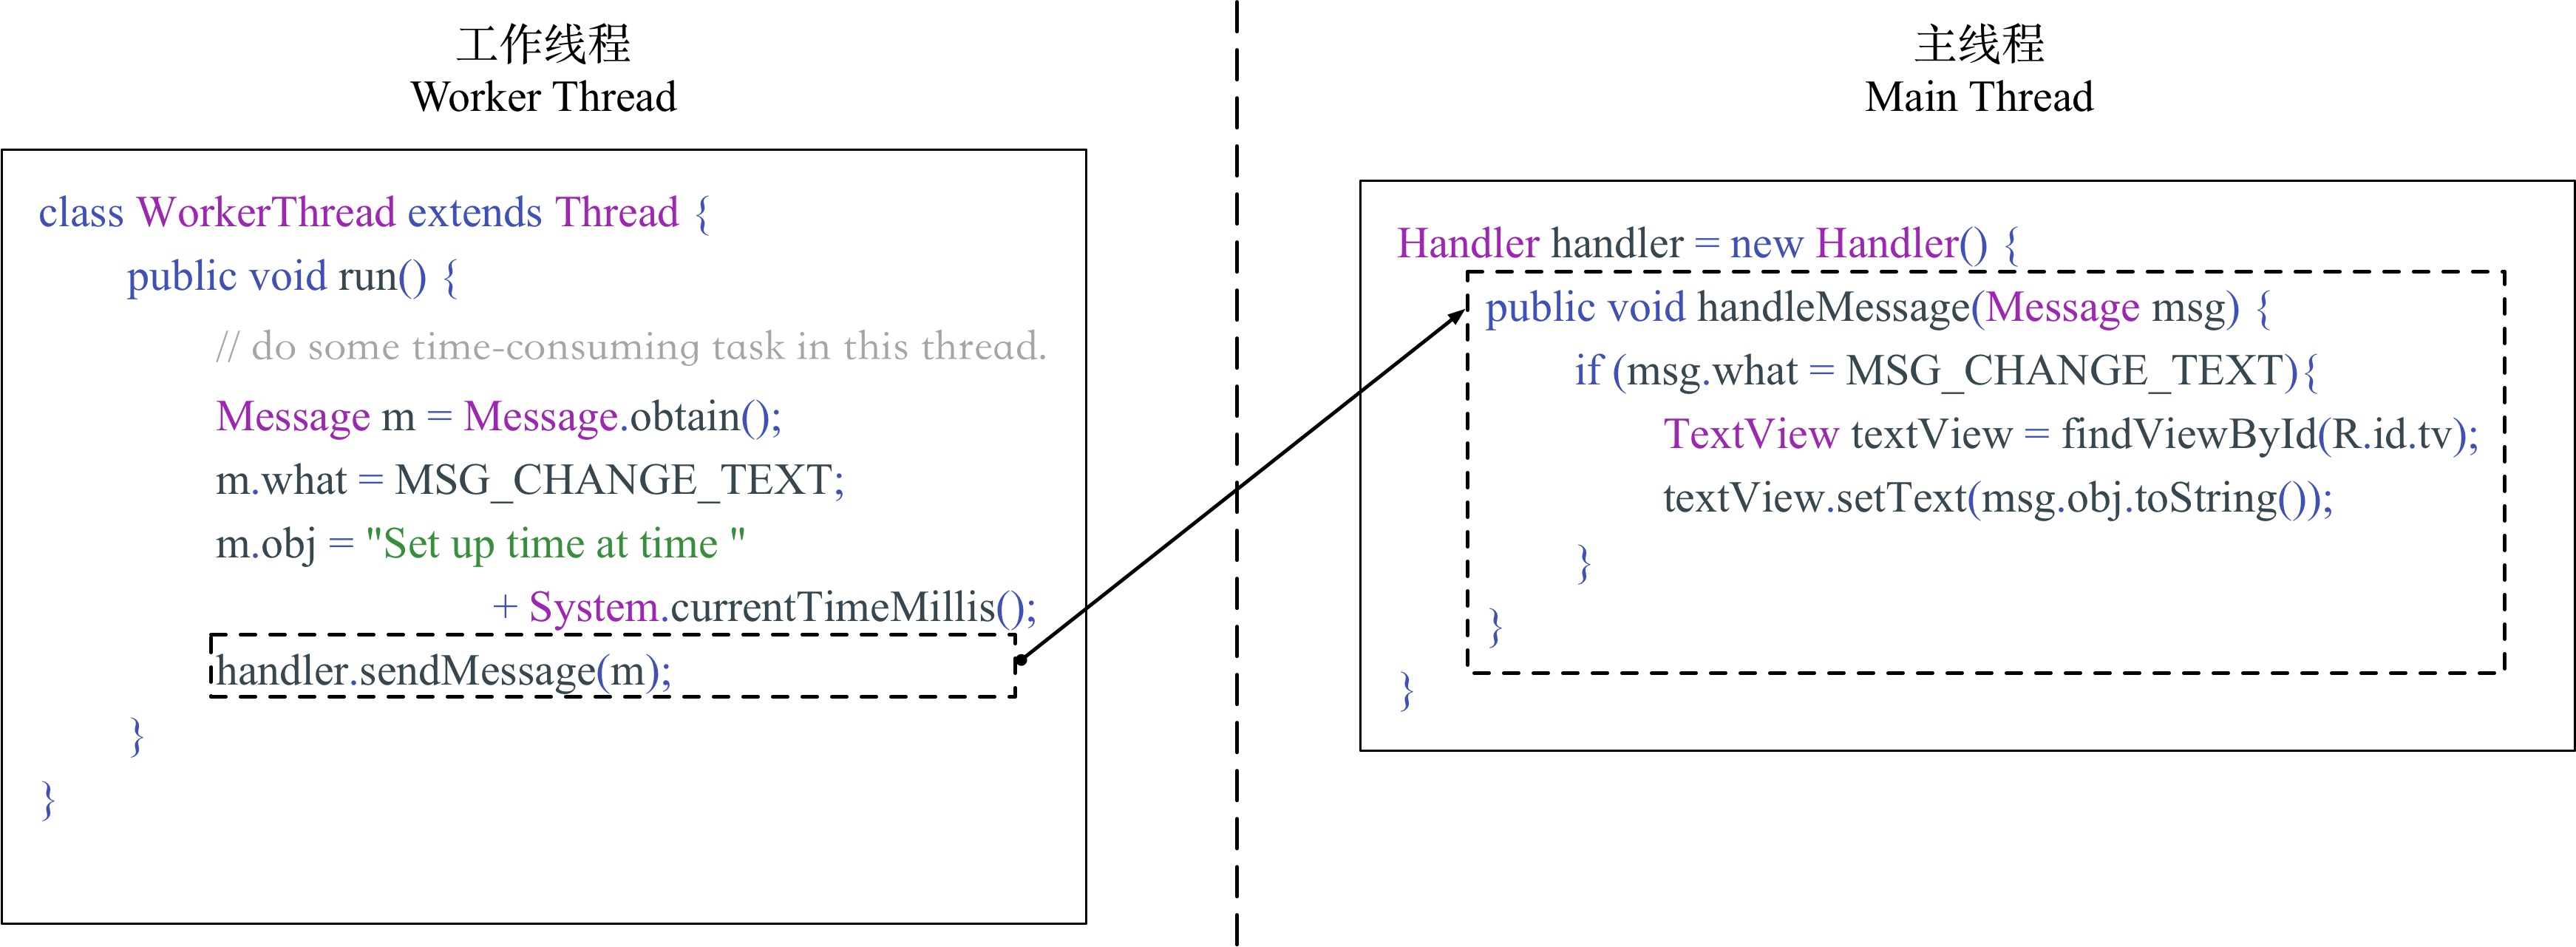
\includegraphics[width=0.9\textwidth]{./Figures/handler-code.png}
	\caption{Handler的使用实例}
	\label{fig:handler-code}
\end{figure*}


\autoref{fig:handler-code}为关于Handler的使用示例。
图中对应的场景为应用由于业务需要获取一个字符串,并将这个字符串展现在用户界面上。
考虑到获取字符串的过程比较耗时,可能会阻塞主线程的相关业务,因此我们会在工作线程执行这部分逻辑(如\autoref{fig:handler-code}-左所示),而在主线程执行信息展现的逻辑(如\autoref{fig:handler-code}-右所示)。
具体的,在工作线程中,用户生成的字符串和对应的逻辑代码\code{MSG\_CHANGE\_TEXT}封装到\code{Message}对象中,通过Handler发送出去;
Handler在主线程中收到了该\code{Message}对象时,会根据逻辑代码(即\code{Message.what}的值)决定进行对应的逻辑处理(本例中,对应逻辑为更新界面信息)。


%用户在工作线程执行生成一个字符串,将生成的字符串传递给Message对象,并通过Handler对象通知主线程进行界面更新。
%当开发人员需要当前业务逻辑转移到其他线程时,通过方法\code{Message.obtain()}获取一个Message,
%或者将对应的参数传递给Message中的参数字段,最后通过Handler对象发送给指定的消息队列。
%当目标线程的消息队列读取到这条消息时,便会在该线程中执行预定的业务逻辑。



\begin{figure*}[hb]
	\centering
	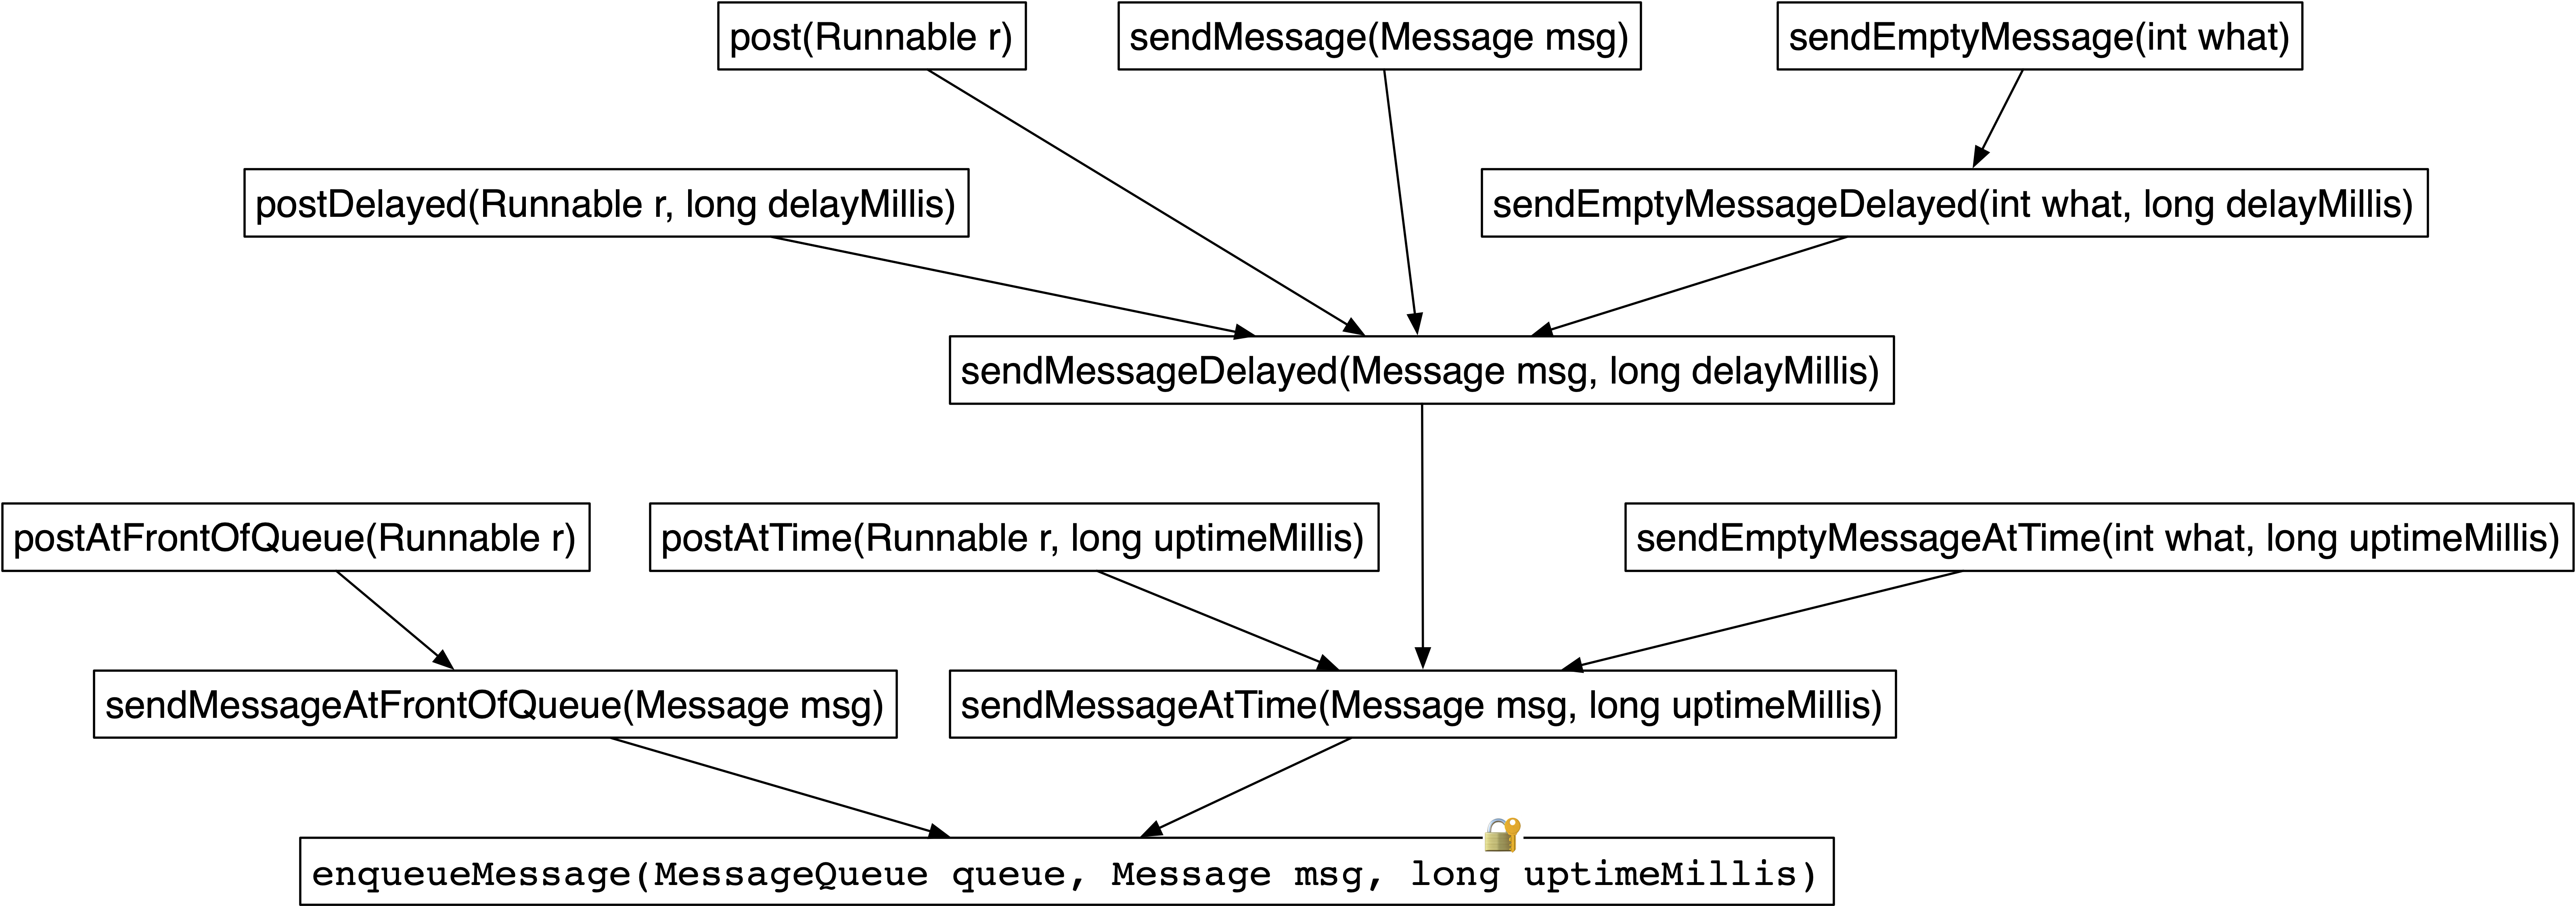
\includegraphics[width=\textwidth]{./Figures/Handler-apis.png}
	\caption{ Handler 各API之间的调用关系}
	\label{fig:handler-apis}
\end{figure*}


除了示例中的调用方式,Android SDK提供的API\cite{HandlerA26:online}还提供多种API(如\autoref{fig:handler-apis}所示),同时支持基于\code{Runnable}的消息调度和基于逻辑代码的消息调度:
%开发人员可以通过\code{post(Runnable)},\code{postAtTime(Runnable,long)},\code{sendMessage(Message)},\code{sendMessageDelayed(Message,long)},\code{sendMessageAtTime(Message,long)}和\code{sendEmptyMessage(int)}等多种API形式实现消息调度。
 通过分析Android系统相关源代码,我们发现上述Handler相关的API关系如\autoref{fig:handler-apis}所示。
从\autoref{fig:handler-apis}中,我们可以发现所有的API最后就会调用到\code{Handler.enqueueMessage( MessageQueue, Message, long)}方法。


Handler机制主要由Handler、Looper、MessageQueue、Message等若干部分组成。
%\begin{enumerate}
%		\setlength{\itemsep}{-5pt}
%\item
 Message是多线程交互的核心载体;
%无论开发人员以何种形式调用了Handler发送消息,相关的参数最后均会被封装到Message对象中。
考虑到移动设备的硬件限制以及Message使用的频繁性,Android系统通过对象池对Message对象进行管理。
%\item 
MessageQueue是一个双端队列,存放所有待处理的Message对象。
%开发人员可以根据具体业务场景在消息队列的头部、尾部或者适当位置插入消息队列。
%\item 
Looper负责消息的分发。
%一个线程最多只允许只有一个Looper对象,他只能绑定一个与之对应的MessageQueue;
%其中最为常见的就是位于主线程的MainLooper,它主要负责Android系统的日常调度(例如Activity的生命周期、控件的点击事件响应等)。
%\item
Handler在整个过程中承担着消息的发送者和消费者两个身份,负责将消息发送到对应的MessageQueue中以及消费来自Looper分发下来的Message。
%在一个应用中,Handler可以存在多个对象,一个Handler对象也可以同时扮演生产者和消费者两个角色。
%\end{enumerate}
Handler机制中各组成部分的相互关系如\autoref{fig:handler-framework}所示。
当用户要通过Handler传递消息时,用户将调用系统提供的Handler API,
该API会将通过分发\code{Handler enqueueMessage(MessageQueue, Message, long)}将消息投递到消息队列MessageQueue中;
当Looper从MessageQueue中读取该Message对象,分发给对应的Handler对象,调用该对象的方法\code{Handler.dispatchMessage(Message)};%使得业务可以在对应恰当的线程上被处理
最终,Handler对象会调用\code{Handler.handleMessage(Message)}按照Message对象进行业务逻辑处理。
\begin{figure*}[!ht]
	\centering
	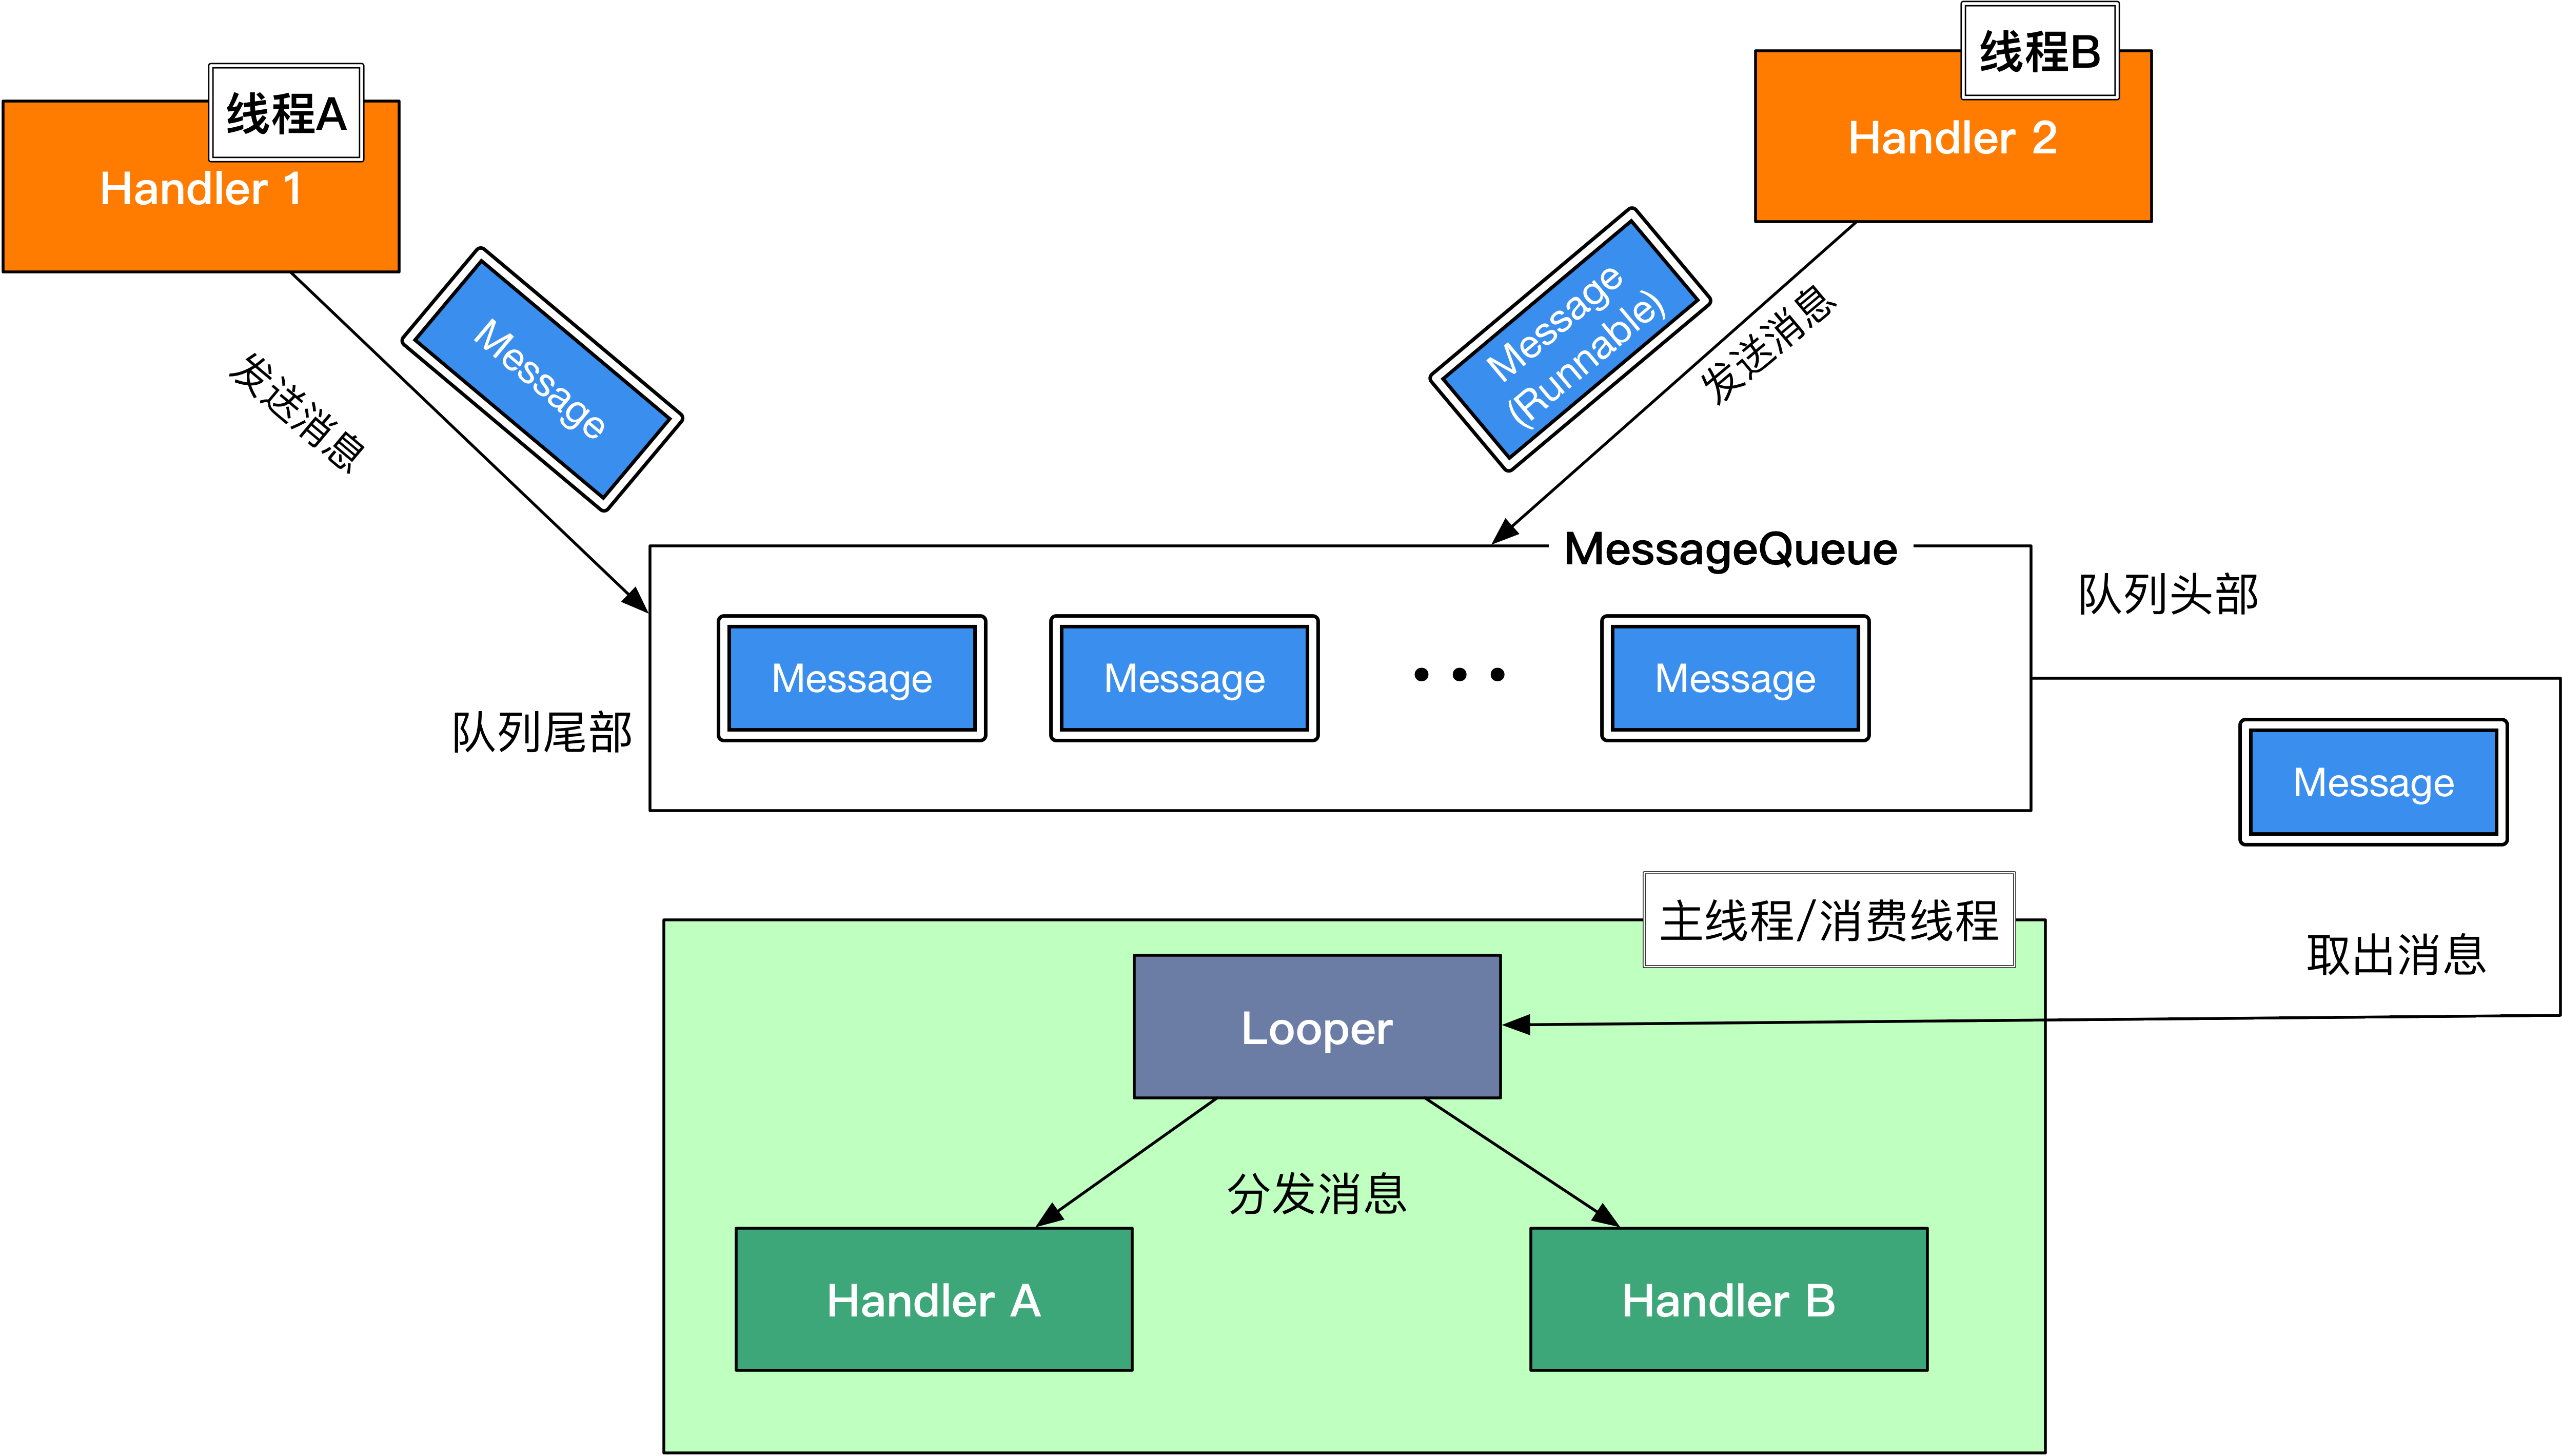
\includegraphics[width=0.8\textwidth]{./Figures/Handler-framework.png}
	\caption{ Handler机制中各组成部分的相互关系}
	\label{fig:handler-framework}
\end{figure*}

基于Handler的多线程消息调度,充分利用了Android的事件驱动架构,将业务逻辑抽象出Message对象,借助消息队列在线程间传递Message,达到了Android多线程交互的目的。
Handler机制,不仅帮助开发人员实现业务逻辑在主线程和工作线程间的自由转移,而且其灵活的API设计降低应用的设计复杂程度,提升了系统架构的可拓展性。
正因如此,在Android开发过程中,基于Handler消息调度的多线程交互十分常见。


\section{本文遇到的困难与挑战}


本文解决的关键问题有如下几点:

1)	如何获取应用程序中各个函数的执行信息?

获取应用程序在执行过程中各函数执行信息是本文的基础。从函数分类上,用户定义的方法和系统预定义的方法。
对于前者,我们可以通过修改程序源代码实现;但对于后者,由于我们无法直接修改系统程序的源代码或者构建一个符合本文业务需求的系统的成本较高,
为此,我们需要寻找对应的解决方案以帮助我们获取系统方法的执行信息。

2)	如何根据程序中各函数的的执行信息,还原应用程序的函数调用图?

基于第一点,我们可以获取程序在运行过程中的执行信息。
但仅仅依靠这些执行信息是不够的,我们还需要将这些执行信息组织起来,挖掘执行信息之间的关联关系,从而才能还原成应用程序的函数调用图。
这将是本文研究的重点之一。

3)	如何在生成的函数调用图中体现Android特性?

正如上文所提的,Android系统中有很多常规应用中不具备的特性,例如Activity的生命周期、基于多线程调用的触发关系。
若要在生成的函数调用图上体现上述特性,需要对Android系统源代码有一定的了解熟悉,并基于图中的相关信息创建与特性相对应的关系。
这既是本文研究的重点,也是本文的创新点。

\section{本章总结}

本章主要介绍了Android系统的相关背景知识,较为详细的阐述了Android的系统结构,详细介绍了Android四大组件之一的Activity生命周期。
同时,本章还介绍了基于Runnable/Thread、Handler消息调度两种不同的多线程交互方式,详细地分析了Handler的运行机制,为下文基于函数调用图的多线程触发关系生成做了铺垫。
最后,本章还介绍了系统在实现上可能遇到的困难。

\clearPaperPage

\chapter{名词解释}
\label{chp:definition}


在本节,我们将给出拓展动态函数调用图构建过程中的基本术语:方法执行、方法对象、调用关系、触发关系、函数调用图、拓展函数调用图等,并将结合具体示例进行解释。

\section{概念说明}
方法执行是一个方法执行相关信息的描述,方法对象对应是和方法执行相关的对象;
调用关系和触发关系描述了方法执行之间的关系。
函数调用图为所有调用关系的集合,在函数调用图上添加方法对象以及触发关系得到拓展函数调用图。相关定义如下:

\subsection{关于方法和对象的定义}

\begin{Def}
	方法对象(Method Object,MO)
\end{Def}

和方法执行相关的对象称为方法对象,可以体现对象和执行方法的相互关系。
在本文中,方法对象通常用符号$o$表示。
	

	对于一个方法执行$m$,对象和方法执行的关系有如下几种:
	\begin{itemize}
%				\setlength{\itemsep}{-5pt}
				\setlength{\itemsep}{1pt}
				\setlength{\parskip}{0pt}
				\setlength{\parsep}{0pt}
		\item 参数关系:若对象$o_p$是这个方法$m$的参数,记为$o_p \joinrel\xrightarrow{parameter} m$;%,或者 $ rel(m,o_p) = parameter$,或者三元组$\left\langle m, o_p, parameter\right\rangle $;
		\item 返回值关系:若对象$o_r$是这个方法$m$的返回值,记为$o_r \joinrel\xrightarrow{return} m$;%,或者 $ rel(m,o_r) = return$,或者三元组$\left\langle m, o_p, return\right\rangle $;
		\item 实例关系:若方法$m$是非静态方法,则方法执行时我们可以获取到关联到的this指针对象$o_i$,记为$o_i \joinrel\xrightarrow{instance} m$。%,或者 $ rel(m,o_i) = instance$,或者三元组$\left\langle m, o_p, instance\right\rangle $;
	\end{itemize}




\begin{Def}方法执行\end{Def}

方法执行是对方法执行过程中的相关信息的描述,完整的信息包括对应方法的完整签名、执行时所处的线程以及相关的方法对象。
在本文中,方法执行通常用符号$m$表示。

\subsection{关于方法间关系的定义}
\begin{Def}
	调用关系(Invoke)
\end{Def}

	对于程序$P$的两个方法$m_1$和$m_2$,方法$m_1$调用了方法$m_2$,则记作$m_1 \to m_2$,称为方法$m_1$调用方法$m_2$。

在此基础上,对于方法$m$,若存在方法$m_i$($i=0,\dots,n , n \geqslant 0$),使得~\autoref{equ:extend_invoke}成立,则记作$m_0 \stackrel{\ast}{\to} m$,称为方法$m_0$扩展调用方法$m_n$。
特殊的,对于方法$m_1$和方法$m_2$,若$m_1 \to m_2$,则$m_1  \stackrel{\ast}{\to}  m_2$也成立。

\begin{equation}
m_0 \to m_1 \to \dots m_n \to m  \label{equ:extend_invoke}
\end{equation}


\important{在系统源代码的层面上},如果对于方法$m$和$m'$,方法$m$的执行过程总是会调用方法$m'$(即$m \to m'$\important{总是}成立),可以记为 $m \Rightarrow m'$;
如果对于方法$m$和$m'$,$m  \stackrel{\ast}{\to}  m'$总是成立,可以记为 $m  \stackrel{\ast}{ \Rightarrow } m'$。

\begin{Def}
	触发关系(Trigger)
\end{Def}
	
	%如果对于动态函数调用图$DCG$中两个方法(不妨记为$m_a$和$m_b$,$m_a \in DCG$,$m_b \in DCG $),
	若方法$m_a$和方法$m_b$之间同时需要满足以下三个条件,
	则两个方法存在触发关系,记为$m_a \hookrightarrow m_b$ 或者$m_{a} \lhook\joinrel\xrightarrow{\text{因果关系}}  m_{b} $,称为$m_a$触发调用$m_b$:
	
	\begin{itemize}
		\setlength{\itemsep}{-5pt}
		\item 方法$m_a$的执行时间总是在方法$m_b$的执行时间之前;
		\item $m_a \stackrel{\ast}{\to} m_b $不成立;
		\item $m_a$、$m_b$之间存在着因果关系,包括但不限于事件回调或多线程交互等。
	\end{itemize}


以多线程中的Thread为例,方法\code{Thread.start()}(记为$m_{start}$)执行会使JVM / Dalvik虚拟机创建一个新的线程。
最终在这个线程中,虚拟机会在新的线程中回调该Thread对象的方法\code{Thread.run()}(记为$m_{run}$)。
上述描述可以表示成$m_{start} \hookrightarrow m_{run}$。由于这个触发关系和多线程相关,也可以记作$m_{start} \lhook\joinrel\xrightarrow{Thread}  m_{run} $。
同样的,触发关系也适用于Ui事件注册与响应、基于Handler的多线程交互。


\important{在系统源代码的层面上},对于方法$m_a$ ,$m_b$ ,$m_c$ ,
若$m_a  \stackrel{\ast}{ \Rightarrow } m_b$ 和 $m_b \hookrightarrow m_c$\important{同时}成立,则$m_a \hookrightarrow m_c$也成立;
若$m_a  \hookrightarrow m_b$ 和 $m_b \stackrel{\ast}{ \Rightarrow }  m_c$\important{同时}成立,则$m_a \hookrightarrow m_c$也成立。

\subsection{关于调用图的定义}

\begin{Def}
	函数调用图(CallGraph,CG)
\end{Def}	

	函数调用图是对程序运行时行为的描述,用有向图$CG = ( V , E)$表示。 图中的点$ v \in V $表示一个\textbf{方法执行} $m$;
	如果方法$m_1$调用方法$m_2$(即$m_1 \to m_2$),则有向边 $e = \left\langle m_1 ,m_2 \right\rangle $属于集合 $E$。 


\textbf{注意:}
在应用执行过程中,方法A被调用了两次,方法A的每次调用都调用了方法B,则对应的函数调用图$CG$如~\autoref{equ:dcg_sample}所示。
在调用图$CG$中,$m_a$ 和 $m_b$ 各有两个,分别对应的两次\textbf{方法执行}。
$\left\langle m_{a_{1}} \to m_{b_{1}}\right\rangle $对应的是第一次函数A调用函数B,
$\left\langle m_{a_{2}} \to m_{b_{2}} \right\rangle    $对应的是第二次函数A调用函数B,

\begin{equation}
\begin{aligned}
CG = &(V,E) ,\\ 
V = & \{m_{a_{1}},m_{b_{1}},m_{a_{2}},m_{b_{2}}\}, \\ 
E = & \{  
\left\langle  m_{a_{1}} \to m_{b_{1}} \right\rangle  ,\left\langle  m_{a_{2}} \to m_{b_{2}}\right\rangle 
\} 
\end{aligned}
\label{equ:dcg_sample} 
\end{equation}



\begin{Def}
	拓展函数调用图(Extended CallGraph,ECG)
\end{Def}


	在函数调用图(CG)的基础上,添加了方法对象和函数间的触发关系。
	拓展函数调用图中的节点包括方法执行节点和方法对象节点。图中的边包括描述方法间关系的边和描述方法和对象间的边:
	前者的方法间关系包括调用关系和触发关系;而后者的关系包括和方法对象相关的三个关系。
	
\eat{
	具体定义如~\autoref{equ:def_edcg}所示:

\begin{equation}
\begin{aligned}
EDCG =              & (V_{EDCG},E_{EDCG}) ,\\ 
DCG =                & (V_{DCG},E_{DCG}) ,\\ 
V_{EDCG} =      & V_{method} \bigcup V_{object} ,\\
V_{method} =   & V_{DCG}, \\ 
G_{EDCG} =      & G_{method} \bigcup G_{object} , \\
G_{method} =  & E_{DCG} \bigcup \{ \left\langle m_1 , m_2 \right\rangle  \mid m_1 \hookrightarrow m_2 \}
\end{aligned}
\label{equ:def_edcg} 
\end{equation}
}
	
	
\section{举例说明}

以第\ref{chp:background}章中的\autoref{fig:handler-code}为例,我们将简要阐述上述概念。
在线程WorkerThread中,方法\code{run()}\eat{$m_{run}$}依次调用了方法\code{Message.obtain()}\eat{$m_{obtain}$}和方法\code{Handler.sendMessage(Message)}\eat{$m_{send}$},则有$m_{run} \to m_{obtain} $和$m_{run} \to m_{send}$。
对于方法$m_{ontain}$,$o_{m} \joinrel\xrightarrow{return} m_{obtain} $成立。
对于方法$m_{send}$,$o_{m} \joinrel\xrightarrow{parameter} m_{send} $、$o_{handler} \joinrel\xrightarrow{instance} m_{send} $成立。
%在Handler的方法handleMessage(Message)中,则有$m_handle \to $
通过对Android Handler 运行机制的分析,我们知道$m_{send} \stackrel{\ast	}{\Rightarrow} m_{enqueue} $、$m_{enqueue} \hookrightarrow m_{dispatch}$以及$m_{dispatch} \stackrel{\ast}{\Rightarrow}  m_{handle}$,
因此,$m_{send} \hookrightarrow m_{handle}$或$m_{send} \lhook\joinrel\xrightarrow{Handler}  m_{handle} $。


\section{本章总结}

本章从方法和对象的关系、方法间关系、调用图等几个方面对方法关系、方法执行、调用关系、触发关系、函数调用图、拓展调用图等概念做了符号化的定义,
并结合第二章的Handler例子简单阐述了上述概念。


\clearPaperPage
\chapter{RunDroid的系统设计}
\label{chp:design}





为了了解Android 应用程序在运行阶段的执行过程,本文提出了一个可用于还原Android应用程序运行时动态函数调用图的工具——RunDroid。
RunDroid利用源程序代码插桩和运行时方法拦截的相结合的方式,捕获应用程序在应用层面和系统层面的方法执行信息,还原方法间的调用关系。
在此基础上,RunDroid利用对象和方法的关系结合具体的触发规则,进而还原出方法间触发关系,在调用图中展现运行过程中的Android特性行为。
RunDroid提供的函数调用图从方法调用关系、方法间的触发关系以及方法执行的相关对象信息等多个方面较为全面地刻画了Android应用程序的执行过程,可以为应用程序分析提供更为多样、准确的信息。


\section{整体设计框架}



\begin{figure*}[!ht]
	\centering
	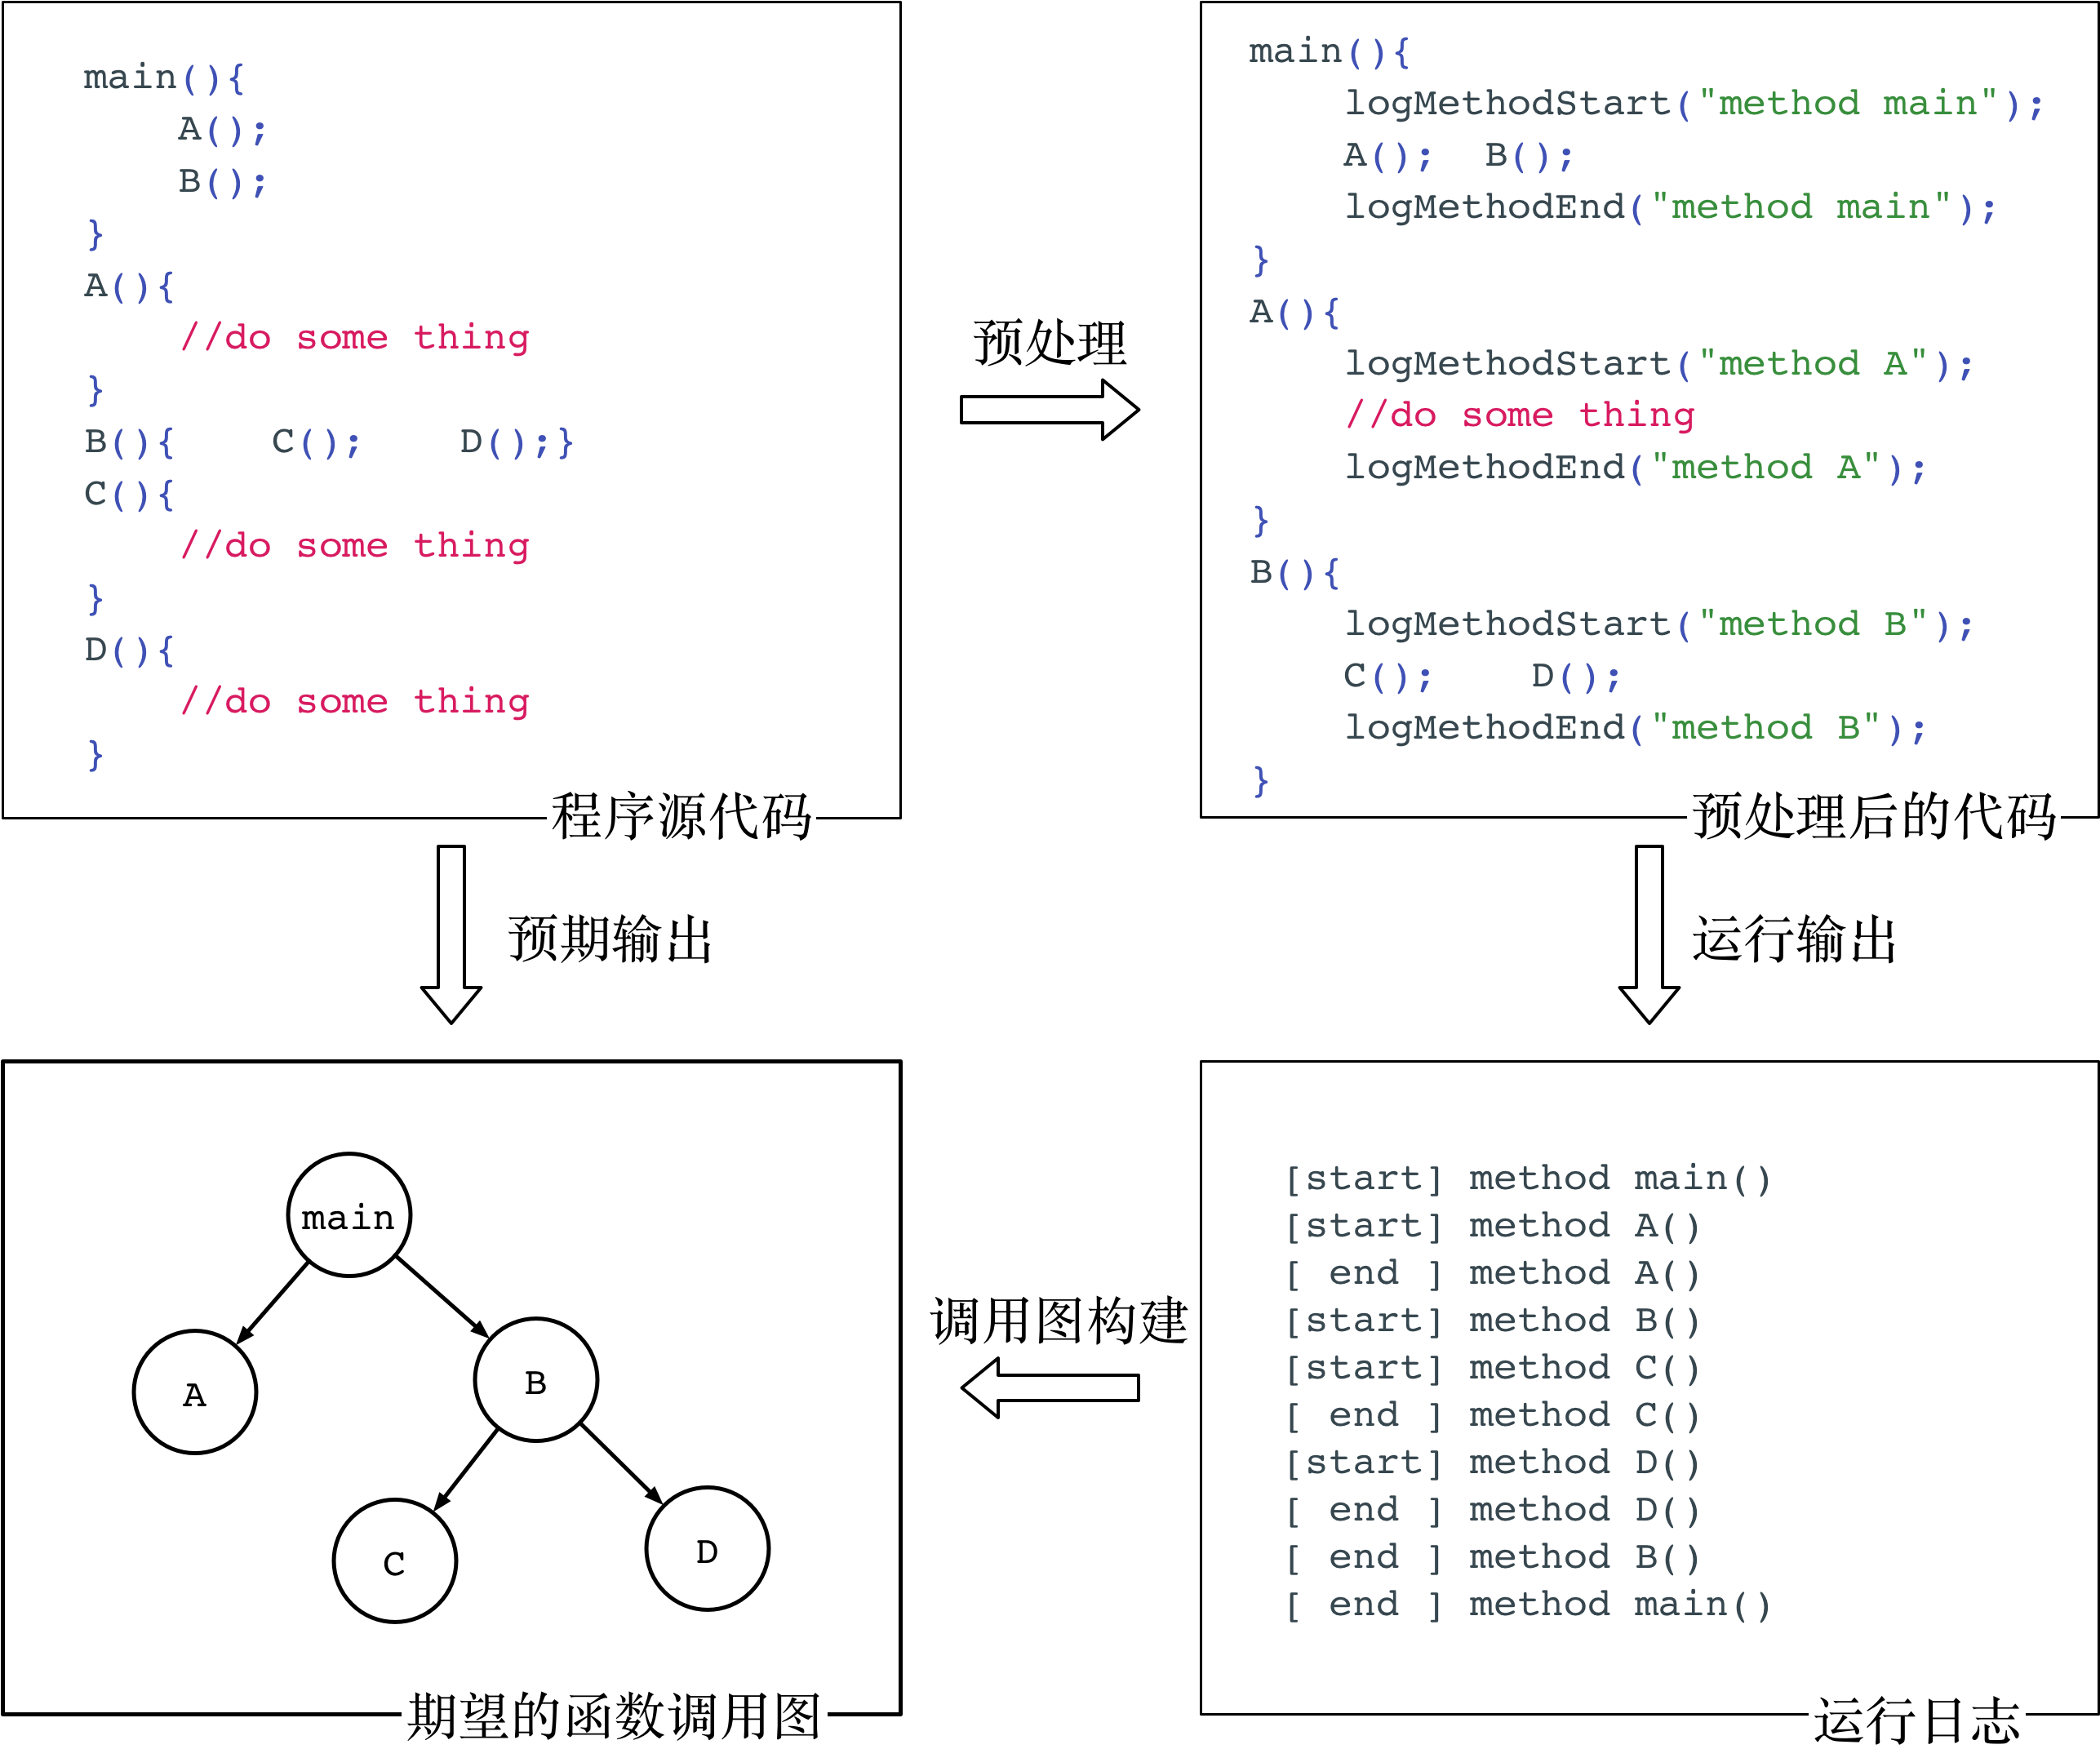
\includegraphics[width=0.8\textwidth]{./Figures/code-sample.png}
	\caption{RunDroid的基本思路}
	\label{fig:code_sample}
\end{figure*}


%在本节,
%以\autoref{fig:code_sample}为例,%简要介绍一下RunDroid还原Android应用程序的函数调用图的基本思路:
\autoref{fig:code_sample}-左上为一段示例代码:在main函数执行时,程序会依次调用A、B两个函数,而B函数则会调用了C、D两个函数。
\autoref{fig:code_sample}-左下则是程序的运行时函数调用图,即RunDroid实际的输出产物。
程序执行过程可以看做函数调用图(树)的深度优先遍历过程\footnote{如果我们将运行过程中一个方法执行看做动态函数调用图中的一个节点,那么,动态函数调用图本身就是一颗树,而不是一个图。}。
还原函数调用图的关键点,在于如何在程序执行过程中输出树的遍历序列,并根据遍历序列进行还原函数调用图。
\eat{
通常的,树的遍历分为中序遍历、前序遍历以及后序遍历三种。
但是,两颗结构完全不同的树对应的遍历序列可能是一样的,
这也就意味着上述三种遍历方法均不能直接还原出函数调用图。
而且,函数执行过程中出现的错误异常可能使得序列输出中断,阻碍调用图的构建。
}
%本文采用的方案是利用在方法执行前后均记录执行日志(即一个方法的执行会输出两条日志:方法开始日志、方法结束日志),
%进行动态函数调用图的还原。

本文采用的方案:
RunDroid通过对源程序(\autoref{fig:code_sample}-左上)进行预处理,得到包含日志记录功能的运行代码(\autoref{fig:code_sample}-右上);
程序在函数执行前后可以输出和方法执行相关的日志信息,(\autoref{fig:code_sample}-右下);
最后,我们根据这些日志信息构建出函数调用图(\autoref{fig:code_sample}-左下)。
另外,在函数调用图的基础上,RunDroid利用日志中包括的方法对象信息,挖掘和方法对象相关联的方法,结合具体触发规则,进而建立方法触发关系。

% 从函数调用图的构建过程可以看出,程序的执行过程就是对函数调用图自上而下的深度优先遍历过程。由此可见,若要还原出图 6-右中的函数调用图,本文采用的基本思路是以日志方式输出对右图中的函数调用图的深度优先遍历序列,并基于得到的遍历序列还原出函数调用图。
% 由于Android是由面向对象编程语言Java开发的系统,系统还需要考虑面向对象编程的特性——多态性(即同一个行为在不同的对象下的表现可以不同)。为此,RunDroid还会在函数调用图将函数执行和对应的对象进行关联,更好地体现面向对象编程的函数调用关系。基于上述的函数调用关系的信息,RunDroid根据函数调用之间的关系进一步挖掘,进一步挖掘Android系统中的特性(例如组件Activity的生命周期、多线程的交互方式)。
%\section{总体框架}


\begin{figure*}[!ht]
	\centering
	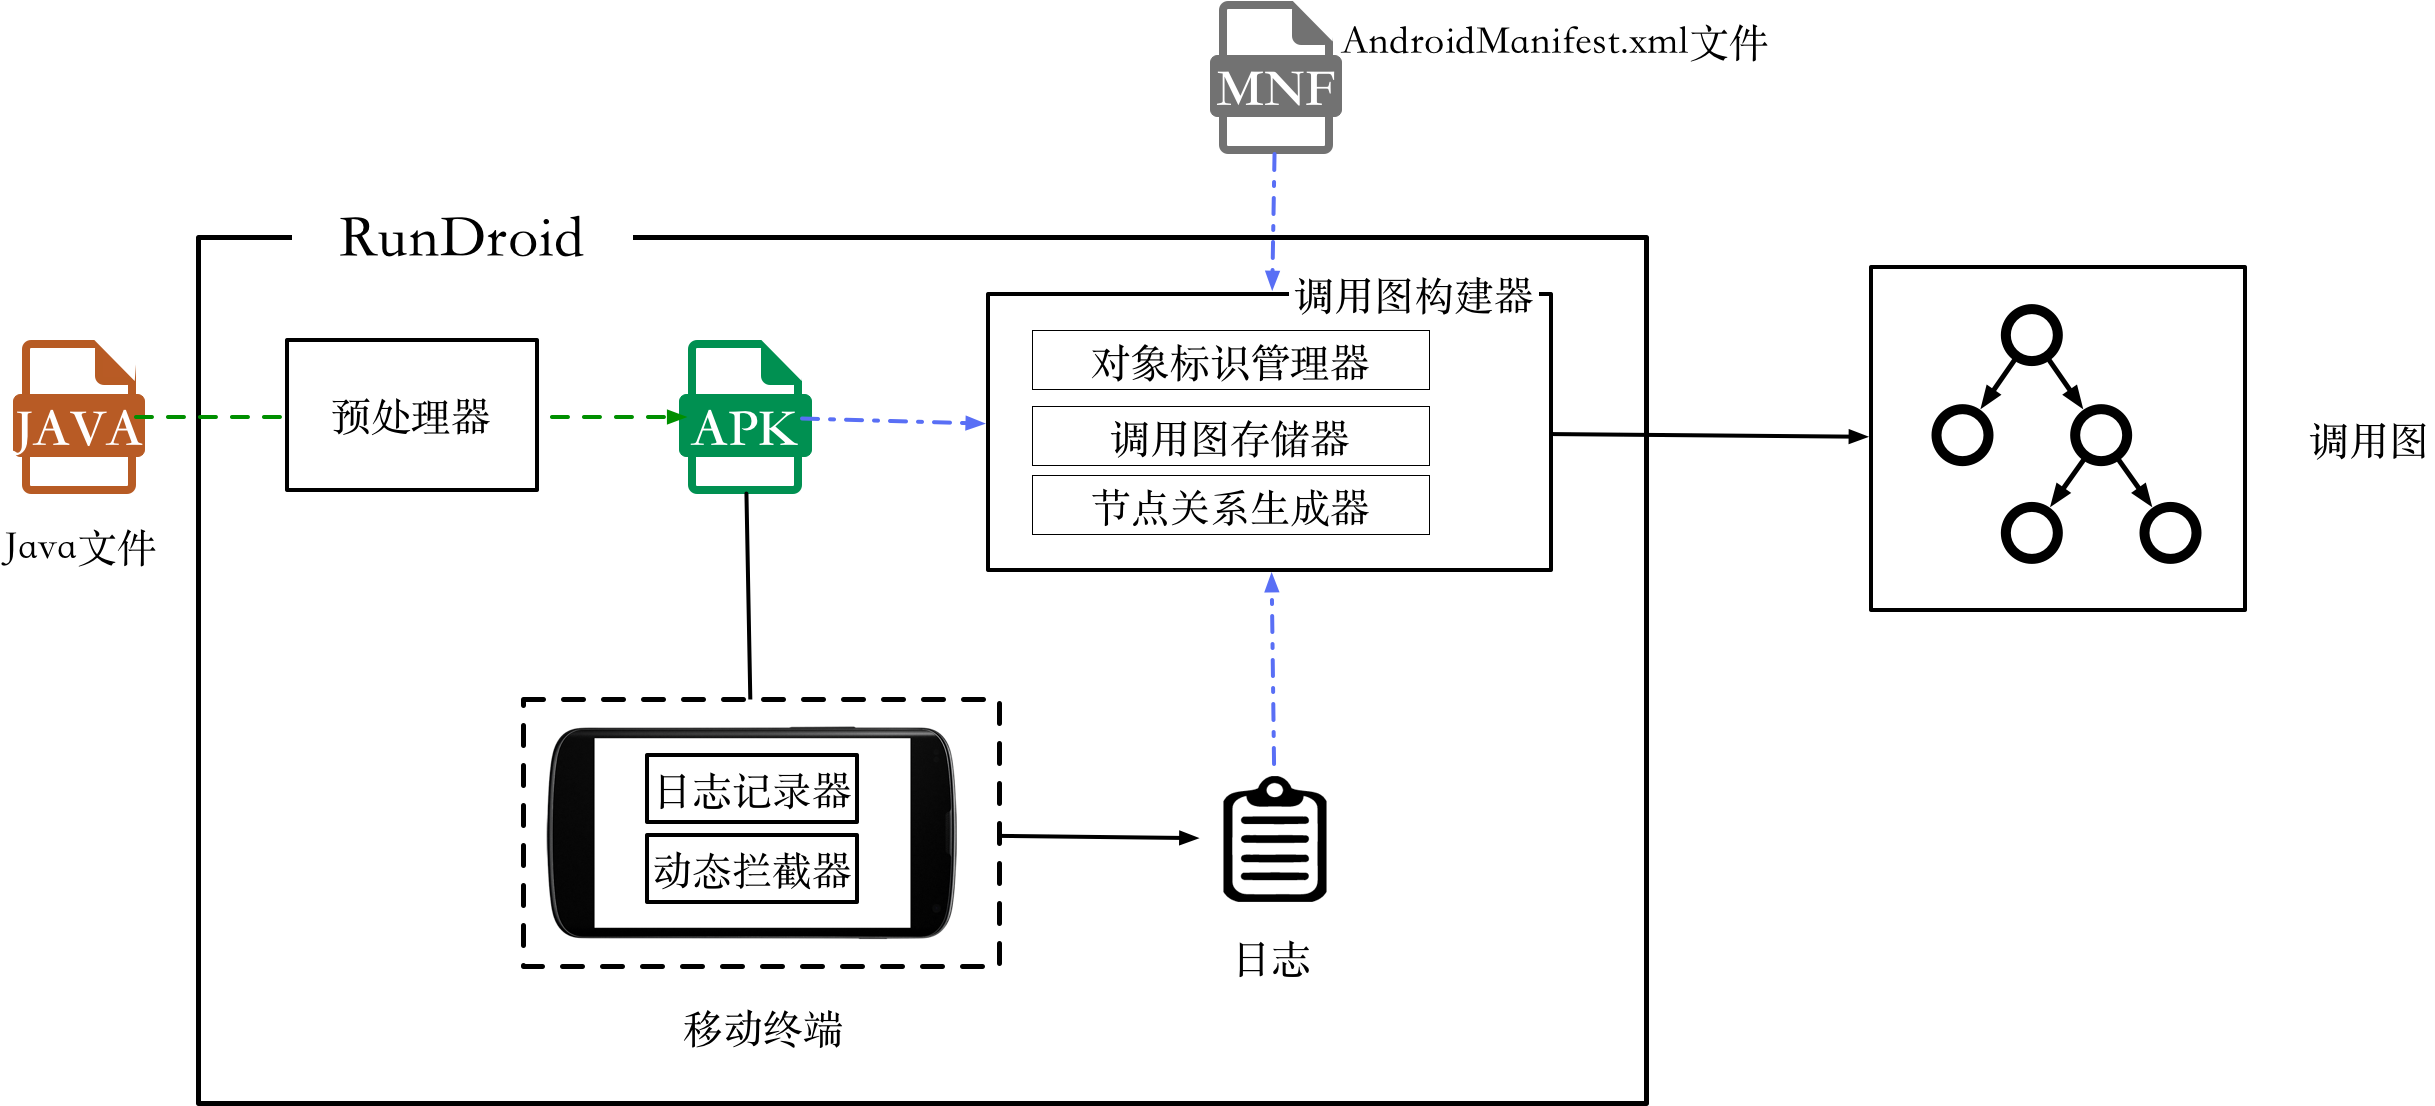
\includegraphics[width=0.8\textwidth]{./Figures/rundroid-overview.png}
	\caption{ RunDroid的工作流程}
	\label{fig:rundroid_overview}
\end{figure*}

在技术实现上,RunDroid主要分为预处理器、运行时拦截器、日志记录器、调用图构建器等4个部分,对应的工作流程如\autoref{fig:rundroid_overview}所示。
从功能上,预处理器和运行时拦截器两者的作用是一致的:在程序运行过程中,当相关方法执行时,触发日志记录器记录相应的信息。
预处理器通过源代码插桩技术实现在用户方法运行时触发用户方法的信息记录,而运行时拦截器则是通过方法劫持技术实现对系统方法执行的拦截,进而触发日志记录。
%系统方法的执行。
%由于,用户方法层面的代码已修改,而系统方法的行为难以修改
%并非所有的方法都是进行日志代码织入的。RunDroid可以接触到用户方法(开发者在应用层面定义的方法)的源代码,而对于前者,
在应用运行时,日志记录器会以日志的形式将用户方法和系统方法对应的执行信息记录下来。
最后,调用图构建器会根据应用程序运行时输出的日志,构建拓展函数调用图。






% 本技术路线拟利用语法分析工具,对Android应用程序进行了应用源代码层面的执行日志插桩工作,利用非侵入式系统行为修改插件获取系统层面的函数执行信息。
% 结合以上日志信息,方案对日志进行初步处理,在图数据库上构建原始的Android应用程序的动态函数调用图。
% 通过阅读分析Android系统中多线程相关的源代码,制定具体的多线程分析插件,进而在函数调用图中标识出多线程相关的方法间触发关系,
%全面地展现Android应用的执行过程。


\section{方法信息的捕获}

在RunDroid中,方法一共分为两类,用户方法和系统方法。
用户方法是由用户定义的,直接修改的成本较低,易于实现。
而系统方法在系统中定义,属于系统运行环境的一部份,行为修改成本较高。
虽然记录这两种方法的执行信息的方式是不一样的。
但是两者最终的效果是一致的:当应用程序运行时,相关方法的执行信息均会通过日志记录器记录下来,用于后续调用图的构建。


\subsection{用户方法执行信息的获取}%——基于源代码的日志代码插桩过程}


预处理器以Android项目源代码作为输入,输出预处理后的APK文件。
%输出的APK文件在应用执行过程中将用户方法的执行信息输出出来。
具体处理过程如\autoref{alg:instrument}所示:
预处理器会遍历项目源代码中的Java源文件,将源文件和对应的抽象语法树转化成XML格式的文件,并以DOM的形式加载到程序中(第1$\sim$4行)。
%  利用获取的语法结构,预处理器会提取出所有的方法体,
对于抽象语法树中的每一个类和每一个方法,预处理器会计算出编译后所处的类的全限类名及方法签名(第5$\sim$\ref{alg:instrument:computeMethodId}行)。
全限类名和方法签名的组合<全限类名,方法签名>可以作为方法体的唯一标识,和抽象语法树中的方法体一一对应。
在每个方法内部,预处理器会插入用户方法日志记录的代码,实现日志代码编织,达到用户方法运行时信息记录的目的(第\ref{alg:instrument:addMethodExitLogCode}$\sim$\ref{alg:instrument:addMethodEnterLogCode}行)。
另外,预处理器还对每个方法体进行了异常捕获处理,防止方法体内部的异常导日志记录过程的中断,影响函数调用图的构建(第\ref{alg:instrument:addMethodCatchLogCode}行)。
上述操作都是对DOM对象\code{document}直接操作的。
当一个Java文件修改完毕后,预处理器会将DOM对象重新转换成Java源文件,并替换原来的文件(第12行)。
最后,预处理器会利用编织后得到的源代码构建成APK文件(第\ref{alg:instrument:buildApk}行)。




\begin{algorithm}[!ht]
	\caption{日志代码插桩过程} 
	\label{alg:instrument}
	\KwIn{ $javaFiles$,应用程序的源代码}
	\KwOut{ $apk$,包含插桩代码的APK文件}
	\SetKwProg{Fn}{Function}{:}{}
	
	\Fn{buildApk($log$)}{
		
		\For{$ javaFile \in javaFiles $}{
			
			transform $javaFile $ to xml-format File $xmlFile$
			
			transform $xmlFile$ to DOM Object $document$
			
			\For{ \emph { $ classEle \in document$}}{
				
				$className \gets $computeClassSign($classEle$,$xmlFile$); 	
				
				\For{\emph { $methodEle \in classEle$}}{
					
					$methodId\gets $computeMethodId($methodEle$,$className$ ); 	 \label{alg:instrument:computeMethodId}
					
					addMethodExitLogCode($methodEle$,$methodId$); \label{alg:instrument:addMethodExitLogCode}
					
					addMethodCatchLogCode($methodEle$,$methodId$);  \label{alg:instrument:addMethodCatchLogCode}
					
					addMethodEnterLogCode($methodEle$,$methodId$); \label{alg:instrument:addMethodEnterLogCode}
				}
				
			}
			write $document$ into new Java File $newJavaFile$
			
		}
		$	apk  \gets$ buildApk($newJavaFiles$)  \label{alg:instrument:buildApk}
		
		\KwRet{apk };
	}
	
\end{algorithm}
\subsection{系统方法执行信息的获取}%——基于动态拦截技术的方法信息捕获}



运行时拦截器的主要职责是对Android系统方法的执行进行拦截,将相关信息传递给日志记录器并记录下来。
运行时拦截器维护着系统方法列表。
列表中的方法通常和Android特性相关,例如Activity的生命周期方法、Java Thread API以及Handler相关的API,具体如\autoref{tbl:hookMethodList}所示。
在目标应用程序开始运行前,运行时拦截器会为上述目标方法注册执行回调函数。
在目标方法执行前和执行后,对应的回调函数会被执行,进而通过日志记录器记录下这些方法执行的相关信息。
在RunDroid中,运行时拦截器可以弥补预处理器无法提供系统方法执行信息的不足,填补调用图缺失的系统方法执行,进而还原出应用层和系统层之间以及系统内部的方法调用,使得产生的调用图更加完整。



\begin{table*}[!ht]
	%	\centering
	\footnotesize		
	
	\caption{运行时拦截器拦截的系统方法列表}
	
	\label{tbl:hookMethodList}
	
	
	\resizebox{\textwidth}{!}{
		\begin{threeparttable}[b]
			
			\begin{tabular}{|l|c|}
				\hline
				方法签名&说明\\
				\hline
				Activity.onCreate(Bundle)   &\multirow{6}{0.4\linewidth}{和Activity生命周期相关的方法}\\
				%	\cline{1-1}
				Activit.onStart()    &\\
				Activity.onResume()     &\\
				Activity.onPause()    &\\	
				Activity.onStop()     &\\
				Activity.onDestroy()    &\\
				\hline
				
				Thread.start()   & 和Java 线程启动相关的方法\\
				\hline
				Message.obtain() & \multirow{15}{0.4\linewidth}{和 Hanlder机制相关的方法}\\
				Handler.enqueueMessage(MessageQueue,Message,long)&\\
				Handler.dispatchMessage(Message)&\\
				Handler.post(Runnable)&\\
				Handler.postAtTime(Runnable,long)&\\
				Handler.postAtTime(Runnable,Object,long)&\\
				Handler.postDelayed(Runnable,long)&\\
				Handler.postAtFrontOfQueue(Runnable)&\\
				Handler.sendMessage(Message)&\\
				Handler.sendEmptyMessage(int)&\\
				Handler.sendEmptyMessageDelayed(int,long)&\\
				Handler.sendEmptyMessageAtTime(int,long)&\\
				Handler.sendMessageAtFrontOfQueue(Message)&\\
				Handler.sendMessageDelayed(Message,long)&\\
				Handler.sendMessageAtTime(Message,long)&\\
				
				\hline
				
				
				%		AsyncTask execute [Object& \multirow{3}{0.4\linewidth}{和 AsyncTask相关的方法}\\
				%		AsyncTask publishProgress [Object&\\
				%		AsyncTask executeOnExecutor Executor [Object &\\
				%		\hline
				
				
			\end{tabular}
			
			%		\begin{tablenote}
			%		\end{tablenote}
			
		\end{threeparttable}
	}
\end{table*}

\section{扩展函数调用图的构建过程}

调用图构建器构建拓展函数调用图的过程分为如下几个阶段:
 RunDroid根据程序运行时的日志提取函数间的调用关系,创建函数调用图;
根据AndroidManifest.xml的Activity组件声明,在函数调用图上标识出完整的Activity 生命周期流转序列;
利用方法执行与方法对象的关联关系,结合触发关系规则,补全方法间的触发关系,形成最终的拓展函数调用图。




\begin{algorithm}[ht]
	\caption{函数调用图的构建过程} 
	\label{alg:buildCG}
	\KwIn{ $logs$,应用程序的运行时日志}
	\KwOut{ $cg$,函数调用图}
	\SetKwProg{Fn}{Function}{:}{}
	
	\Fn{buildCallGraph($log$)}{
		
		$cg$ $\gets$ new CallGraph();
		
		\For{thread $\in$ $logs.threads$}{
			
			$stack$ $\gets$ new Stack();
			
			\For  {$log$ $\in$ $logs.get(thread)$}{
				
				$top$ = $stack$.peek() ;  
				
				\eIf{isMethodStartLog($log$)} {
					
					$m \gets $ generateMethodInfo($log$);
					
					$cg$.addMethodNode($m$);
					%\Comment 在调用图中提交方法节点 
					
					$cg$.addMethodObjectsIfNotExists($ o_p $,$o_i $) 	;							
					
					$cg$.addMethodObjectRels($ \left\langle  o_p \joinrel\xrightarrow{parameter}   m \right\rangle   $,$ \left\langle  o_i \joinrel\xrightarrow{instance}   m \right\rangle  $) ;
					
					%	\Comment 在调用图中提交方法对象节点 (此处只涉及参数关系和实例关系)
					
					\If {  $top \neq null $ }{
						
						$cg$.addInvokeRel($ \left\langle  top \to  m \right\rangle  $) ;
						
						$stack$.push($m$);
					}
					
				}{ 
					
					$cg$.addMethodObjectIfNotExists($  o_r  $) ;
					
					$cg$.addMethodObjectRel($ \left\langle   o_r \joinrel\xrightarrow{return}   m \right\rangle  $) ;
					
					%		  \Comment 在调用图中提交方法对象节点 (此处只涉及返回值关系)
					
					$stack$.pop() ;
					
				}
				
				
				
			}
		}
		\KwRet{ $cg$};
	}
	
\end{algorithm}
\subsection{构建函数调用图}

%虽然所有线程的方法日志输入到同一个文件中,但是,从单个线程的视角看这些日志,日志在时间维度上的先后顺序就是对调用图的深度遍历。
%已检测的应用程序将日志输出到单个文件中。
%虽然所有线程的日志都输出到一个日志文件中,但在每个线程的视图中,日志条目的输出顺序遵循调用图的顺序遍历:调用方法在被调用方法之前输出。
%此外,每个方法执行对应于两个日志条目:方法入口和出口的日志条目。

由于各个线程在执行过程中,不存在一个调用关系跨越两个线程,因此,在整个构建过程中,RunDroid以产生日志的线程为基本构建单元,向调用图添加方法调用关系。
函数调用图的构建过程如\autoref{alg:buildCG}所示。

对于每个线程,RunDroid顺序遍历对应的日志,使用栈$stack$的入栈、出栈操作来模拟对应线程的函数执行的过程,还原调用关系(第2$\sim$ 20行):
当读取到方法执行的开始日志时,系统会在调用图创建一个节点表示该方法的执行(第7$\sim$8行),
同时也在调用图中添加方法参数、方法实例对应的对象节点$o_p$、$o_i$以及方法对象和方法的关系$ \left\langle  o_p \joinrel\xrightarrow{parameter}   m \right\rangle   $、$ \left\langle   o_i \joinrel\xrightarrow{instance}   m \right\rangle  $(第9$\sim$10行)。
如果此时当前线程栈$stack$的栈顶方法元素$top$存在,系统会创建从方法$top$到当前方法$m$的调用关系,$\left\langle top \to m \right \rangle  $,并将当前方法$m$压入栈$stack$中(第11$\sim$ 14行)。
当读取到方法执行的结束日志时,该日志对应的方法必然是栈顶方法$top$,若栈顶方法$top$存在返回对象$o_r$,则只需要将$o_r$和$top$的关系添加到调用图中即可,最后弹出栈顶的$top$即可(第 16$\sim$ 18行)。
在上述过程中,如果待添加的方法对象在调用图中已经存在时,该对象则无须重新添加,只需添加方法与对象间的关系即可。




% 当日志条目表示方法条目时,将根据日志条目和来自的4元组信息创建节点 日志存储在节点中(第6行)。
%然后,从堆栈顶部的方法到日志条目中的方法(第7-9行)构建调用关系。
%处理完调用关系后,该方法将被推入堆栈。当日志条目表示方法退出时,堆栈将弹出顶部的方法节点(第11-12行)。
%重复该过程,直到没有为一个线程留下日志条目,然后将为日志文件中的另一个线程启动相同的进程。

%构建扩展调用图。 
%DROIDSTITCHER通过添加表示已识别触发关系的边来扩展调用图。
%请注意,触发器关系中的目标方法通常是回调方法的调用图的入口点。
%因此,通过将触发关系添加为边,将所有调用图拼接成一个调用图作为输出。



\subsection{构建Activity的生命周期和事件回调}

\point{构建Activity的生命周期}

Android 应用的Acticvity生命周期的构建就是将Activity生命周期方法按照时间顺序串联起来,利用的是\code{Activity}生命周期方法的签名的不变性。

\begin{algorithm}[!ht]
	\caption{构建Activity的生命周期和事件回调} 
	\label{alg:buildActivityLifecycle}
	\KwIn{ $manifestFile$,AndroidManifest文件}
	\KwIn{ $cg$,函数调用图}	
	\KwOut{ $cg'$,包括Activity生命周期的函数调用图}
	
	
	
	\SetKwProg{Fn}{Function}{:}{}
	
		\Fn{patchActivityLifecycleAndUiEvent($cg$)}{
		
		patchActivityLifecycle($cg$,$manifestFile$);
		
		patchUiEvent($cg$);
		
		
		$cg' \gets cg$;

		\KwRet{$cg'$};
	}
	
	
	\Fn{patchActivityLifecycle($cg$,$manifestFile$)}{
		
		
		$lifecycleList \gets$ new   $ List()$;
		
		
		\For{ \emph{ $o_{activity} \in \{ activity \mid activity $ defined in  $manifestFile \} $ }}{
			
			
			
			\For{ \emph{ $m \in \{ m \mid  m$ is method node in $ cg $   
					and $o_{activity}$ is instance of $m\}$}}{
				
				
				\If{ \emph{ $m$ is the method of Activity's Lifecycle   \\\qquad
						and  Thread for $m$ is MainThread	  \\\qquad
						and $  \left\langle  m' \to m \right\rangle  \notin cg$
				} }{
					
					$lifecycleList$.add($m$);
				}
				
				
			}
		}
		
		sortListByTime($lifecycleList$);
		
		linkItemsByTime($lifecycleList$,$cg$);
		
	}
	% $o_p \stackrel{parameter}{\longrightarrow} m$
	\Fn{patchUiEvent($cg$)} {
		\For{\emph{$o_{listener} \in \{ o \mid o $  is the $View.OnClickListener$ object node ,$o \in$ $cg \}$} }{
			\If{ {$ \left\langle m_{register}\joinrel\xrightarrow{instance} o_{listener}\right\rangle \in cg$ } \\\qquad 
				and   {$\left\langle m_{click} \joinrel\xrightarrow{instance}   o_{listener}\right\rangle  \in cg$ }}{
				$cg$.addTriggerRel($m_{register} \lhook\joinrel\xrightarrow{UiEvent}  m_{click} $)	
			}
		}
	}		
\end{algorithm}

整个过程以AndroidManifest文件作为输入,在原有的函数调用图的基础上,添加表示Activity生命周期的有向边,具体过程如\autoref{alg:buildActivityLifecycle}所示:
对于AndroidManifest文件中声明的每一个Activity组件$o_{activity}$,系统都会遍历以该对象为方法实例的方法$m$(即$m$、$o_{activity}$满足条件$o_{activity} \joinrel\xrightarrow{instance} m$);
若方法$m$同时满足三个条件,则将它添加到列表$lifecycleList$中(第3$\sim$8行)。
最后,将列表$lifecycleList$按照时间顺序进行排序,并依次连接起来,即可得到\code{Activity}的生命周期(第9$\sim$10行)。

这三个条件分别为:
(1)方法$m$的方法签名和\autoref{fig:Activity-lifecycle}中的任何一个生命周期方法的签名保持一致;
(2)方法$m$执行时所处的线程为主线程;
(3)方法$m$在调用图$cg$中不在调用者,即在调用图$cg$中不存在方法$m' \in cg$,使得$m' \to m $成立。


\point{\todo{Andoid事件回调的触发关系}}



 \subsection{构建多线程触发关系}
基于函数调用图构建多线程触发关系主要分为两个方面,基于Java 的多线程交互与基于\code{Handler} 的多线程消息调度,具体的过程如\autoref{alg:buildTrigger}所示。



\begin{algorithm}[!ht]
	\caption{扩展函数调用图的构建过程}
	\label{alg:buildTrigger}
	\KwIn {	$cg$, 函数调用图} 
	\KwOut {	$ecg$,拓展函数调用图}
	
	
	\SetKwProg{Fn}{Function}{:}{}
	\Fn{buildExtendedCallGraph($cg$)}{
		
		$ecg \gets cg$;
		
		addThreadTrigger($ecg$);
		
		addHandlerTrigger($ecg$);
		
		\KwRet $ecg$;
	}
	
	% $o_p \stackrel{parameter}{\longrightarrow} m$
	\Fn{addThreadTrigger($ecg$)} {
		\For{\emph{$o_r \in \{ o \mid o $  is the $Runnable$ object node ,$o \in$ $ecg \}$} }{
			\If{ {$ \left\langle m_{start}\joinrel\xrightarrow{instance} o_r \right\rangle \in ecg$ } \\\qquad 
				and   {$\left\langle m_{run} \joinrel\xrightarrow{instance}   o_r\right\rangle  \in ecg$ }}{
				$ecg$.addTriggerRel($m_{start} \lhook\joinrel\xrightarrow{Thread}  m_{run} $)	
			}
			\If{ {$ \left\langle m_{runOnUiThread} \joinrel\xrightarrow{parameter}   o_r \right\rangle \in ecg$}  \\\qquad   
				and  { $\left\langle m_{run} \joinrel\xrightarrow{instance}   o_r\right\rangle  \in ecg$  }}{
				$ecg$.addTriggerRel($m_{runOnUiThread}  \lhook\joinrel\xrightarrow{runOnUiThread}  m_{run} $)	
			}	
		}
	}	
	\Fn{addHandlerTrigger($ecg$)} {
		
		\For{\emph{ $o_m \in  \{ o\mid$ o is the $Message$ object node ,$o \in$ $ecg \}$} }{
			\If{{ $ \left\langle m_{enqueue}\joinrel\xrightarrow{parameter} o_m\right\rangle \in ecg$}  \\\qquad   
				and  { $\left\langle m_{dispatch}\joinrel\xrightarrow{parameter} o_m\right\rangle  \in ecg$ }}{
				$m_{send}$ =  calculateSendMethod($ecg$,$m_{enqueue}$);
				
				$m_{handle}$ =  calculateHandleMethod($ecg$,$m_{dispatch}$);
				
				$ecg$.addTriggerRel($m_{send} \lhook\joinrel\xrightarrow{Handler} m_{handle} $ )	
			}	
		}
	}
	
\end{algorithm}
\point{基于Java 的多线程交互}

基于Java的多线程交互往往是以\code{Runnable}作为传递对象,通常通过调用方法\code{Thread.start()} (用$m_{start}$表示)和\code{Activity.runOnUiThread(Runnable)}(用$m_{runOnUiThread}$表示)等API,进而触发方法\code{Runnable.run()}(用$m_{run}$表示)的执行。
因此,对于方法\code{Thread.start()},如果存在一个\code{Runnable}类型的对象\code{r},它既是方法$m_{start}$的实例,又是方法$m_{run}$的实例,则两个方法间存在触发关系,即$m_{start} \hookrightarrow m_{run}$(第8 $\sim$10行)。
同样的,对于方法\code{Activity.runOnUiThread(Runnable)},也存在类似的关系:
如果存在一个\code{Runnable}类型的对象\code{r},它既是方法$m_{runOnUiThread}$的参数,又是方法$m_{run}$的实例,则两个方法间存在触发关系,即$m_{runOnUiThread} \hookrightarrow m_{run}$(第11 $\sim$13行)。

\eat{\begin{equation}
	\label{equ:rule_1}
	\left. \begin{gathered}
	o_r    \        is           \      Runnable  \      Class \\
	rel(m_{start}, o_r) = instance \\
	rel(m_{run}, o_r) = instance \\
	\end{gathered} \right\}
	\Rightarrow  m_{start} \hookrightarrow m_{run}. 
	\end{equation}
}
\eat{
\begin{equation}
\label{equ:rule_2}
\left. \begin{gathered}
o_r    \        is           \      Runnable  \      Class \\
rel(m_{runOnUiThread}, o_r) = parameter \\
rel(m_{run}, o_r) = instance \\
\end{gathered} \right\}
\Rightarrow  m_{runOnUiThread} \hookrightarrow m_{run}. 
\end{equation}
}








\point{基于\code{Handler} 的多线程消息调度}

根据第\ref{chp:background}、\ref{chp:definition}章的介绍,我们已经知晓用户通过调用Handler提供的API,
将相关业务逻辑借助Message对象传递给目标线程的Handler对象,在目标线程执行相应的业务逻辑处理。
%在这个部分,我们需要找出用户调用的Handler API和对应目标线程的业务逻辑方法间的触发关系:
首先,我们利用类\code{Handler}的方法\code{enqueueMessage(Message)}(用$m_{enqueue}$表示)和\code{dispatchMessage(Message)}(用$m_{dispatch}$表示)公用同一个Message对象的特点,
找到所有的Handler底层函数触发关系 ,$m_{enqueue}  \hookrightarrow  m_{dispatch}$ (第16$\sim$17 行);
对于每一个触发关系 $m_{enqueue}  \hookrightarrow  m_{dispatch}$,
从$m_{enqueue}$ 顺着调用关系往上找到最上层的Handler API方法(即用户调用的Handler API方法,$m_{send}$)(第18行),
从$m_{dispatch}$ 顺着调用关系往下找到用户定义的方法\code{Handler.handleMessage(Message)}$m_{handle}$(第19行),
最后在调用图中提交方法$m_{send}$和$m_{handle}$之间的触发关系 $m_{send} \lhook\joinrel\xrightarrow{Handler} m_{handle}$(第20行)。
%如果$m_{send}$和$m_{handle}$中有一个方法未找到,表示


\eat{
MATCH (SEND:METHOD)-[:PARAM]->(MSG:OBJECT),

(SEND:METHOD)-[:INSTANCE]->(HANDLER:OBJECT),

(HANDLE:METHOD)-[:PARAM]->(MSG:OBJECT),

(HANDLE:METHOD)-[:INSTANCE]->(HANDLER:OBJECT)

WHERE SEND.methodSign ='boolean android.os.Handler.enqueueMessage(android.os.MessageQueue,android.os.Message,long)'

AND HANDLE.methodSign ='void android.os.Handler.dispatchMessage(android.os.Message)'

RETURN SEND,HANDLE
	
	
	
	
MATCH p=(method:METHOD)-[:INVOKE*0..]->(enqueue:METHOD),

(enqueue)-[:TRIGGER\_PREPARE\_HANDLER]->(dispatch:METHOD)

AND  NOT (enqueue)-[:INVOKE]->()

RETURN p,method,enqueue,dispatch;

	
	
MATCH p=(method:METHOD)-[:INVOKE*0..]->(enqueue:METHOD),

(enqueue)-[:TRIGGER\_PREPARE\_HANDLER]->(dispatch:METHOD)-[r:INVOKE]->(run:METHOD)

WHERE method.methodSign IN [

'boolean android.os.Handler.post(java.lang.Runnable)',

'boolean android.os.Handler.postAtTime(java.lang.Runnable,long)',

'boolean android.os.Handler.postAtTime(java.lang.Runnable,java.lang.Object,long)',

'boolean android.os.Handler.postDelayed(java.lang.Runnable,long)']

RETURN p,method,enqueue,dispatch, run

	
	
	
MATCH p=(method:METHOD)-[:INVOKE*0..]->(enqueue:METHOD),

(enqueue)-[:TRIGGER\_PREPARE\_HANDLER]->(dispatch:METHOD)

AND  NOT (enqueue)-[:INVOKE]->()

RETURN p,method,enqueue,dispatch

	

}

\eat{识别触发关系。
触发关系表示由于Android框架的生命周期事件,系统事件和多线程通信而导致的方法的隐式调用。
以Handler为例。 sendMessage方法隐式意味着稍后将执行相应的方法handlerMessage。
为了捕获这种关系,我们确定了一种模式:sendMessage方法通过传递消息对象来触发方法handlerMessage。
因此,如果我们可以找到用作方法sendMessage和方法handlerMessage的参数的消息对象,那么我们可以在这两个方法之间创建触发器关系。
在分析了Android框架的源代码之后,我们确定了线程,窗口小部件的侦听器注册和异步任务的类似模式。
因此,DROIDSTITCHER维护一个方法列表,这些方法是触发器关系的潜在目标,并比较这些方法中消息对象的内存地址以推断关系。
}



 \section{本章总结}

本章详细介绍了RunDroid的设计。
首先,本章简要介绍了RunDroid实现的基本功能,并通过一个简单的例子介绍了RunDroid的整体运行框架。
由此,我们提出了RunDroid技术路线:RunDroid利用源代码插桩和运行时拦截器相结合的方式,将运行时的方法执行信息以日志的形式保存下来,通过线程内部各个方法日志的嵌套关系还原出函数调用图,并在此基础上构建Activity的生命周期,补全方法间的触发关系,形成最终的拓展函数调用图。


\cleardoublepage

\chapter{RunDroid的系统实现 }

\label{chp:implement}

\eat{

RunDroid使用Java作为开发语言,使用了srcML、Xposed、Neo4j等技术,由预处理器、运行时拦截器、日志记录器、调用图构建器等部分组成。
本章将详细的介绍上述技术及RunDroid各组成部分的实现细节。
}



在技术实现上,RunDroid主要分为预处理器、运行时拦截器、日志记录器、调用图构建器等4个部分,整体架构图如\autoref{fig:rundroid_overview}所示。
%从功能上,预处理器和运行时拦截器两者的作用是一致的:在程序运行过程中,当相关方法执行时,触发日志记录器记录相应的信息。
预处理器通过源代码插桩技术实现在用户方法运行时触发用户方法的信息记录,而运行时拦截器则是通过方法劫持技术实现对系统方法执行的拦截,进而触发日志记录。
%系统方法的执行。
%由于,用户方法层面的代码已修改,而系统方法的行为难以修改
%并非所有的方法都是进行日志代码织入的。RunDroid可以接触到用户方法(开发者在应用层面定义的方法)的源代码,而对于前者,
在应用运行时,日志记录器会以日志的形式将用户方法和系统方法对应的执行信息记录下来。
最后,调用图构建器会根据应用程序运行时输出的日志,构建拓展函数调用图。

\begin{figure*}[!hb]
	\centering
	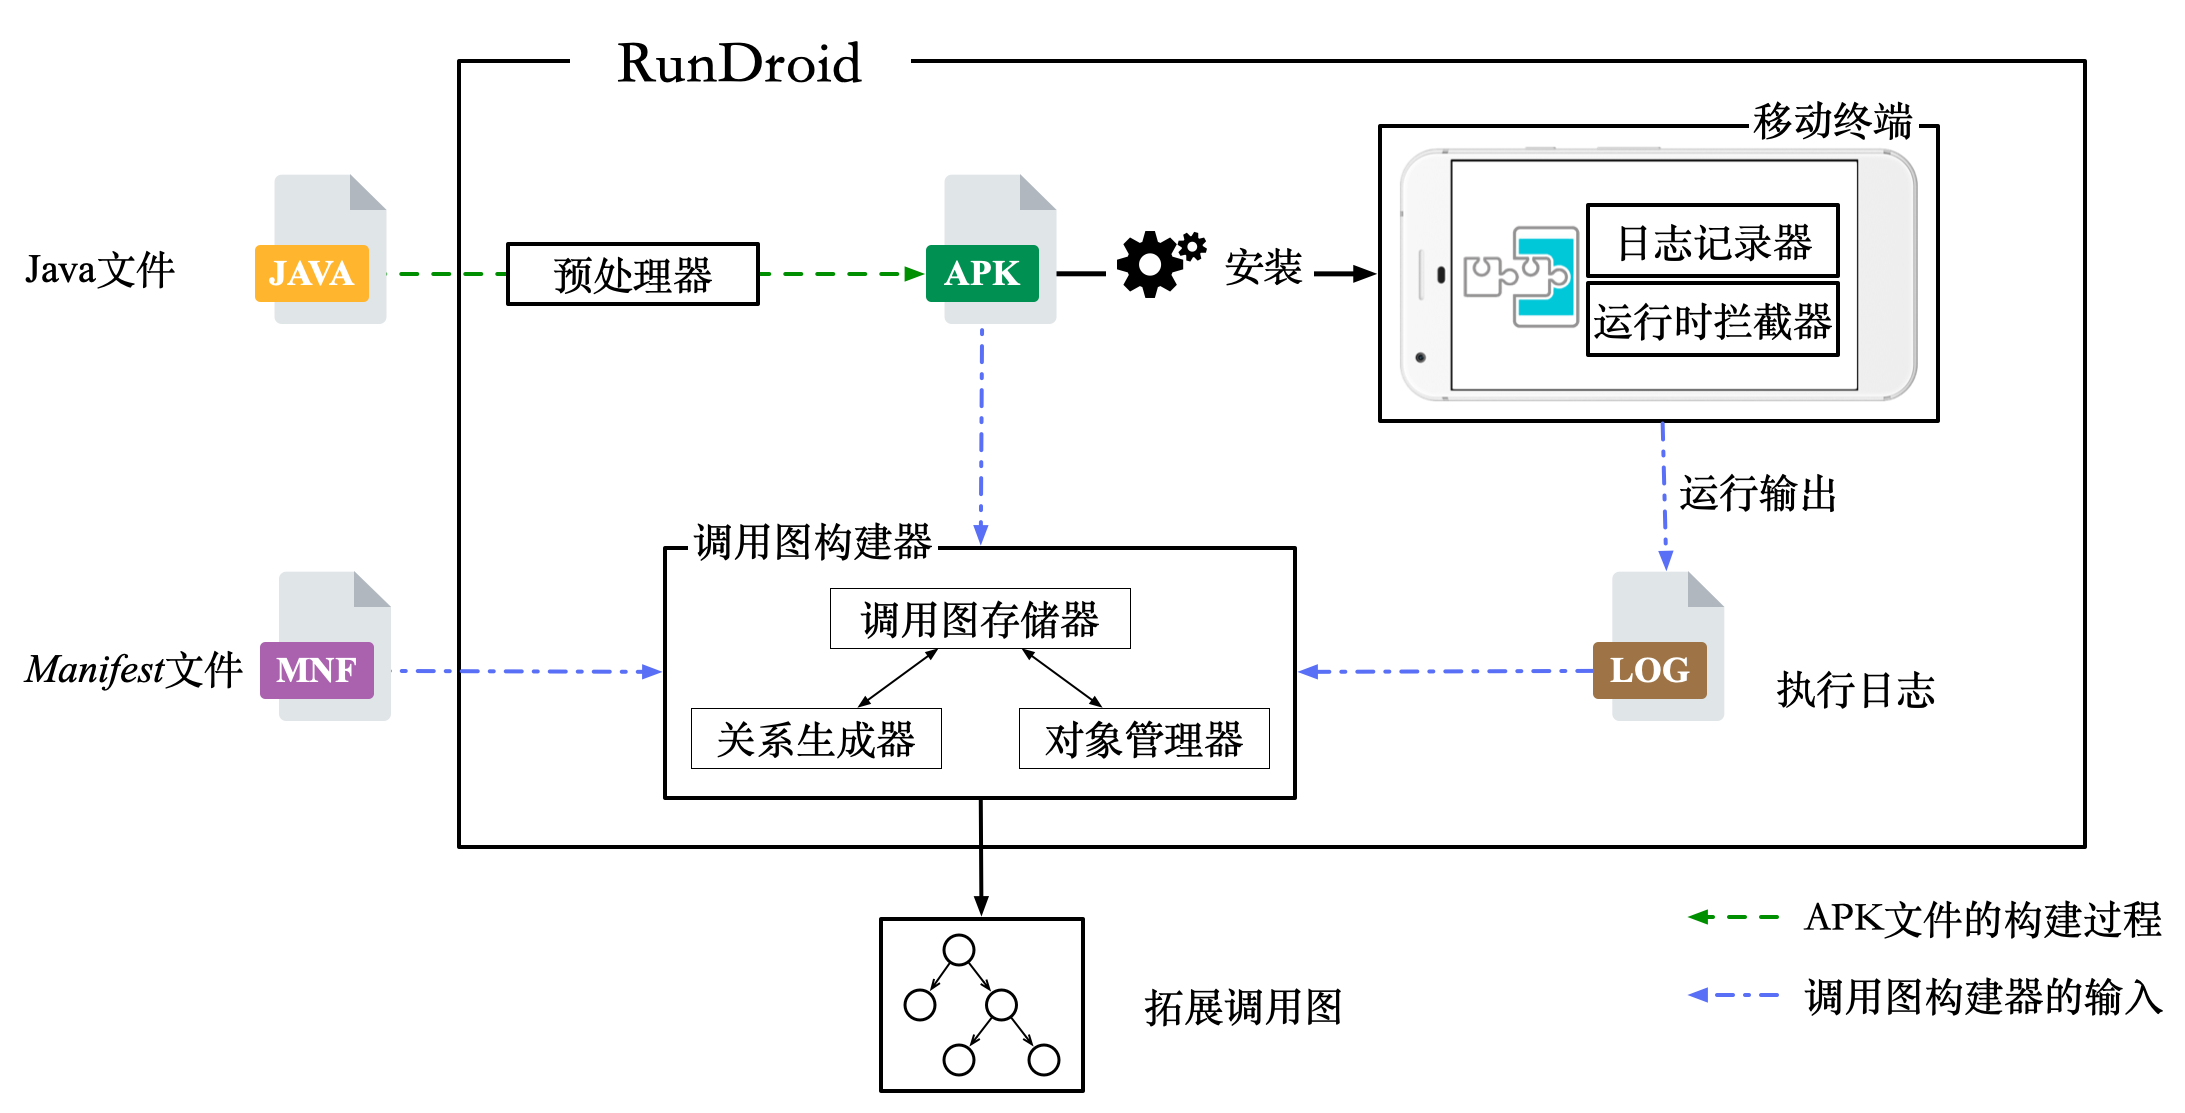
\includegraphics[width=0.8\textwidth]{./Figures/overview.png}
	\caption{ RunDroid的整体架构图}
	\label{fig:rundroid_overview}
\end{figure*}


\section{模块实现}



\subsection{预处理器}

预处理器在RunDroid中的作用主要是用户方法的日志代码编织。
在现有的技术上,代码编织主要分为两类:基于源代码的代码编织和基于字节码的代码编织。
字节码编织技术以AspectJ\cite{TheAspecJ}为典型代表,技术成熟,应用广泛。
但是,字节码插桩技术在运行过程中会生成过多的方法数,在Android应用构建过程中可能存在方法数65K限制问题。
为此,预处理器采用的方案是基于源代码的代码编织方案。

在实现上,预处理器利用轻量级源代码分析工具srcML\cite{collard2013srcml}对程序的源代码进行语法解析,将程序的抽象语法树转化成XML文件。
在XML文件的基础上,预处理器直接对每个方法体进行修改,实现日志代码的编织,最后重新转换成源代码,经过构建得到可以运行的APK文件。
该方案通过直接修改源程序,将日志记录代码写入在方法体内部,避免了新方法的引入,规避了方法数65K限制问题。

%它可以,支持C、C++、C\#以及Java等多个语言的语法解析。
%	同时,srcML还提供了一个强大工具集,支持对生成内容的查询、分析以及修改,可以用于架构设计、语言研究、软件重构等场景,应用于软件工程、编程语言、并行和分布式处理等多个领域。
%在RunDroid,srcML作为RunDroid预处理器中的重要组成部分,承担源代码语法解析的主要职责,辅助完成用户方法层面的日志代码的编织。
% 拦截器组件基于Xposed框架[5],它拦截在应用程序层和Android框架之间传递的消息。
% 拦截器记录在两个层之间进行的每个方法调用,并将它们与应用程序层中对应的方法调用相关联,以产生完整的方法调用跟踪。
% RunDroid维护感兴趣的方法列表,如生命周期方法和隐式回调,以便日志文件包含每次执行期间调用的方法调用

\subsection{运行时拦截器}%——系统方法的捕获}

%由于预处理器可以处理的方法需要
由于无法对系统方法的源代码进行直接修改,因此预处理器无法实现对系统方法的日志代码编织,无法达到系统方法信息记录的目的。
为了弥补预处理器的不足,RunDroid中的运行时拦截器需要在系统层面上实现对系统方法的拦截,实现后续方法信息的日志记录。


%Interceptor组件构建在Xposed框架[5]之上,它拦截在应用程序层和Android框架之间传递的消息。 
%Interceptor记录在两个层之间进行的每个方法调用,并将它们与应用程序层中的相应方法调用相关联,以生成完整的方法调用跟踪。
 %RunDroid维护一组感兴趣的方法,例如生命周期方法和隐式回调,以便日志文件包含每次执行期间调用的方法调用。

%xposed是一个模块框架,可以在不接触任何APKs的情况下改变系统和应用程序的行为。这很棒,因为这意味着模块可以在不做任何改变的情况下为不同版本甚至是rom工作(只要原始代码没有太多改变)。撤销也很容易。由于所有更改都在内存中完成,您只需关闭模块并重新启动即可恢复原始系统。还有许多其他优点,但这里还有一个:多个模块可以对系统或应用程序的同一部分进行更改。有了改进的APKs,你可以选择一个。除非作者用不同的组合构建多个APKs,否则无法将它们组合起来。


%posed是一个基于Android系统的运行时行为修改框架。
%在不修改程序源代码的情况下,基于Xposed开发的第三方插件通过将目标方法关联到函数执行回调上,进行方法参数和返回值的重写和额外方法逻辑的添加等操作,达到目标方法行为修改的目的。
%	Xposed的实现原理具体如下:由于Android系统的所有的应用程序进程都是由Zygote进程孵化而来,Xposed通过替换程序\code{/system/bin/app\_process},使得系统在启动程中加载Xposed的相关文件,将所有的目标方法指向Native方法xposedCallHandler,维护目标方法和对应的钩子方法(Hook Function)的映射关系,从而实现对Zygote进程及Dalvik虚拟机的劫持;
% 当程序执行到目标方法时,xposedCallHandler会完成目标方法的原有代码和对应钩子方法的调度,达到对目标方法劫持的目的。
%利用Xposed提供的类似面向切面编程的API接口,RunDroid中的运行时拦截器可以对任意方法(包括用户方法和系统方法)执行过程进行动态拦截,达到系统方法信息的日志记录的目的。


在实现上,运行时拦截器是基于Xposed\cite{Xposed}实现的插件,它维护的列表包括了所有需要拦截的系统方法。%,如\autoref{tbl:hookMethodList} 所示。
每当目标应用程序启动时,运行时拦截器通过Xposed提供的API\code{ XposedHelpers.findAndHookMethod()}将\autoref{tbl:hookMethodList}中的目标方法绑定到方法钩子(即\eat{Xposed提供的XC\_MethodHook的子类 ,}类HookCallBack)上。
在应用程序的运行过程中,HookCallBack对象的方法\code{beforeHookedMethod(MethodHookParam)}会在目标方法执行之前被调用,
方法\code{afterHookedMethod(MethodHookParam)}会在目标方法执行后调用。
上述两个方法的参数\code{MethodHookParam}中会包括该方法执行时的相关方法对象。
最终,HookCallBack对应会将方法执行的相关信息传递给日志记录器。



相比定制化Android系统,通过Xposed实现的运行时拦截器兼容性良好,适用于市面上主流的Android系统版本,实现成本低。
同时,待拦截方法列表的编辑功能的引入,使得在不修改插件代码的情况下,支持动态添加删除待拦截的方法,避免了Xposed插件修改后的系统重启操作,提高了RunDroid整体的执行效率。
 

\subsection{日志记录器}

日志记录器的职责是将方法执行的消息以日志文件的形式进行持久化存储。
针对不同的方法类型(静态方法与非静态方法、用户方法与系统方法等),日志记录器提供了不同的API,帮助我们记录相应方法执行的日志信息。
在日志内容上,日志记录器还会记录每个方法执行的时间戳、所处线程、方法签名标识、所处阶段(方法开始执行阶段/方法执行完毕阶段)以及相关的方法对象信息。
方法对象信息主要包括对象的类型、属性和全局ID(通过Java API\code{System.identityHashCode(Object)}获取)等。
同时,日志记录器还支持对象信息的自定义:开发人员可以根据自身的需要为不同类型的对象输出不同对象数据信息。
% 在底层实现上,考虑日志读入文件对程序执行效率的影响,我们评估了多种日志写入方式,最终我们发现基于mmap的日志记录方式效率最高,对程序运行的影响最小。




\subsection{调用图构建器}

% 调用图构建器的功能是拓展函数调用图的构建、存储和展现。
调用图构建器由调用图存储器、对象管理器和关系生成器组成,如\autoref{fig:rundroid_overview}所示。

调用图存储器将Neo4j\cite{Neo4jthe19}作为调用图的存储引擎,承担着拓展函数调用图的存储、查询、展示的职责。
Neo4j的数据分为节点和关系两种类型,支持自定义键值属性。
同时,Neo4j可为节点指定标签,为关系指定类型,用于区分不同含义的节点和关系。
拓展函数调用图中的数据在Neo4j中的表现形式如下:
调用图中的方法和对象会以节点的形式出现在调用图中, 方法节点的标签分为\code{METHOD}和\code{FRAMEWORK},对象节点的标签为\code{OBJECT};
方法间关系分为调用关系和触发关系,分别用关系\code{INVOKE}和\code{TRIGGER}表示;
方法和对象之间的关系分为参数关系、返回值关系和实例关系,分别用关系\code{PARAMETER}、\code{RETURN}、\code{INSTANCE}表示。




\eat{
	Neo4j是基于Java语言开发的图数据库,可以用于存储图结构相关的数据结构。
	%与传统的基于关系模型的存储结构不同,Neo4j的存储模型是基于图论开发的,遵循属性图数据模型。


	在数据操作接口方面,Neo4j支持Cypher、Java API和RESTful API等方式,提供友好的数据浏览界面用于数据的展示与修改。
	\eat{由于基于属性图数据模型,Neo4j通常适用于和图关系有着密切关系的应用场景:例如社交网络分析,公共交通网络研究以及地图网络拓扑等场景。}
	在RunDroid,Neo4j是调用图构建器的主要组成部分,承担着拓展函数调用图的存储、查询、展示的职责。
}


对象管理器负责将日志中的对象信息映射成调用图中的节点。
通常情况下,我们认为对象和全局ID一一对应,所以,我们将全局ID相同的对象信息映射成调用图中的一个节点。
但考虑到有些类型(例如Handler机制中的Message)使用对象池技术,我们还在全局ID的基础上引入对象版本号,避免对象在不同生命周期的串用。
以Message为例,调用图构建过程中,如果对象管理器发现待提交的Message对象$m$是方法\code{Message.obtain()}的返回值,处理逻辑如下:
如果调用图中不存在一个全局ID和$m$一致的节点,则对象管理器会创建一个全新的节点来表示$m$,设置其对象版本号为1;
而调用图已经存在一个全局ID和$m$一致,版本号为$version$的节点$m'$,则对象管理器会创建一个全新的节点来表示$m$,并将$version + 1$作为节点$m$的版本号,而不是复用原有节点象$m'$。
因此,在对象管理器的角度看来,两个Message对象只有当全局ID和对象版本号都一致时,才是同一个对象。



关系生成器是\autoref{alg:buildCG}、\autoref{alg:buildActivityLifecycle}、\autoref{alg:buildTrigger}的具体实现,由Cypher脚本和Soot等技术共同实现。
当我们需要找到使用$o_{m}$作为参数的方法$m_{enqueue}$、$m_{dispatch}$(\autoref{alg:buildTrigger}第11行)时,可以直接使用脚本\autoref{fig:cypher_code}
直接在调用图中找到所有符合条件的节点。
相比传统的编程语言,Cypher在实现相同逻辑时,表达形式简洁,代码可读性高,开发效率高效。
Soot的工作主要是提供应用程序相关的类继承检索服务。
例如,\autoref{alg:buildTrigger}第7行中,我们需要知道所有的Runnable对象,此处便需要通过Soot查询所有的Runnable子类。
在算法\ref{alg:buildActivityLifecycle}中,我们也会将Soot和Cypher相结合用于查找所有Activity的生命周期方法。


\begin{figure}[!h]
	\centering
	%normal
	\begin{lstlisting}[style=normal,language=cypher]
	MATCH (m_enqueue:METHOD)-[:PARAM]->(o_m:OBJECT),
					(m_dispatch:METHOD)-[:PARAM]->(o_m:OBJECT)
	return o_m, m_enqueue, m_dispatch\end{lstlisting}
	\caption{使用Cypher查找共用对象$o_m$的方法$m_{enqueue}$、$m_{dispatch}$}
	\label{fig:cypher_code}
\end{figure}


 \section{本章总结}

本章侧重介绍RunDroid的系统实现。
在整体上,RunDroid由预处理器、运行时拦截器、日志记录器、调用图构建器等部分组成。
预处理器和运行时拦截器分别对应应用程序在执行过程中用户方法和系统方法的执行拦截,以触发日志记录器记录方法执行信息。
预处理器是通过源代码编织实现的,避免了新方法的引入,规避了方法数65K限制问题。
运行时拦截器借助Xposed框架提供的方法执行劫持技术实现对系统方法的执行拦截,在实现上规避了Xposed插件修改后的重启系统操作。
调用图构建器将运行过程中方法执行的日志信息作为输入,在Neo4j图数据库上构建函数调用图,利用图中方法和对象之间的关系,利用Soot和Cypher语句实现Activity生命周期的构建、方法触发关系的生成,形成最终的扩展函数调用图。

\clearPaperPage
\chapter{系统测试}  
\label{chp:testing}


\section{实验简介}
\section{构建效率对比实验}
\section{日志效率对比实验}
\section{运行效率对比实验}
 \section{本章小结}

\clearPaperPage
\input{chapter-application.tex}

\clearPaperPage

\chapter{总结与展望}
\label{chp:future}
\section{总结}

本文尝试提出一个Android动态函数调用图构建系统,从应用层和系统层对Android应用程序的执行过程进行记录,并利用得到的执行日志信息还原Android应用程序的动态函数调用图,从方法层面还原程序的执行过程。
另外,通过Android系统的源代码进行分析,我们可以找到Android应用程序中多线程相关的函数触发关系,进一步全面的展现Android应用程序的执行过程。
另外,开发人员还可以对系统进行拓展,实现自身的需求。
\section{展望}



\clearPaperPage
	\addcontentsline{toc}{chapter}{参考文献}
	\bibliographystyle{GBT7714-2005}
	\bibliography{bib/tex}

 \eat{
\clearPaperPage


\fancypagestyle{plain}{%
	\fancyhead[LE,RO]{华东师范大学硕士专业学位论文}
	\fancyhead[RE,LO]{ 致  谢}
}


\addcontentsline{toc}{chapter}{致  谢}

{\kaishu
{\chapter*{\vspace{-3cm} 致\qquad 谢}}

\vspace{-0.5cm}

\begin{center} 
\end{center}
	
	在此论文完成之际,我首先要感谢我的导师杜德慧。她严肃的科学态度,严谨的治学精神以及精益求精的工作作风深深地感染和激励着我。从课题的选择到项目的最终完成,杜老师都始终给予我细心的指导和不懈的支持。两年来,她不仅在学业上给我以精心指导,同时还在思想、生活上给我以无微不至的关怀与照顾,在此谨向杜老师致以诚挚的谢意和崇高的敬意。

	感谢在研究生学习期间给我诸多教诲和帮助的软件学院的各位老师和同学、以及和我一起生活两年的室友,你们的执着、勤奋、以及对生活的态度,值得我学习。特别的,我要感谢辅导员张炜帆对我思想以及生活上的帮助,给我带来了莫大的帮助。

	最后感谢我的家人,你们不仅给我经济上的支持,同时还在我成长道路上无私地给予莫大支持与鼓励,让我独立地选择自己的人生道路。

\vspace{0.2cm} \hspace{11.5cm} 

\hspace{10.6cm}  二〇一七年十月 }

}
\clearPaperPage


\fancypagestyle{plain}{%
	\fancyhead[LE,RO]{华东师范大学硕士专业学位论文}
	\fancyhead[RE,LO]{ 攻读学位期间发表的学术论文}
}



\addcontentsline{toc}{chapter}{攻读学位期间发表的学术论文}
\section*{攻读硕士学位期间发表论文}

\vskip 5mm

{\heiti $\blacksquare$ 已公开发表论文}\vskip 5mm

\begin{enumerate}

  \item Yujie Yuan, Lihua Xu, Xusheng Xiao, Andy Podgurski, and Huibiao Zhu,RunDroid: Recovering Execution Call Graphs for Android Applications. In Proc. ESEC/FSE, 2017
  \eat{
  	\item xxxx  Proceedings of the IEEE Conference on Computer Vision and Pattern Recognition xxxxx 为模式识别和计算机视觉的三大国际顶级会议,中国计算机协会列为A类会议,根据猲猰猱猷年谷歌学术统计,h5-index排名所有学术刊物第35位,位列工程和计算机领域所有学术刊物第一位。 
  	注:第二作者,导师第一作者。xxxx是中国计算机协 会A类、图像处理领域的顶级期刊,SCI II区。
  }

\end{enumerate}






\end{document}

